\documentclass[a4paper,12pt,openany]{report}
\usepackage[utf8]{inputenc}  %pour utiliser les mots avec accents
\usepackage[T1]{fontenc}   % utiliser tous les caractères du clavier
\usepackage[french]{layout}  % pour paramétrer les marges du document
\usepackage{here}
\usepackage{latexsym}  %Pour utiliser divers symboles mathématiques
\usepackage{textcomp}
\usepackage{amsfonts}        %pour gerer le fond des couleurs
\usepackage{amssymb}         %POUR GERER LES FORMULES ET EXPRESSIONS MATHEMATIQUES
\usepackage{amsthm}         %POUR GERER LES FORMULES ET EXPRESSIONS MATHEMATIQUES
\usepackage{mathrsfs}
\usepackage[centertags]{amsmath}   %POUR GERER LES FORMULES ET EXPRESSIONS MATHEMATIQUES
\usepackage{fancyhdr}        %Pour personnaliser l'en-tête et pied de page
\usepackage[dvips]{epsfig}
\usepackage{color}     %pour colorer du texte dans le document
\usepackage{float}
\usepackage{times}
\usepackage{shadow} %pour gerer les ombres
\usepackage{txfonts}
%\usepackage[colorlinks, citecolor=blue]{hyperref}
\usepackage[french]{babel}
\usepackage{graphicx}    %Pour inserer des images
\usepackage{colortbl}
\usepackage{fancybox}           %Pour GERER LES BOX ET ENCADREMENTS
\usepackage{rotating}
\usepackage[left=2cm, right=2cm, top=2.5cm, bottom=2.5cm]{geometry} %POUR la taille des marges
\pagestyle{headings}
\usepackage{slashbox}       %Pour SCINDER LES CASES DU TABLEAU
\usepackage{framed}
\usepackage{sectsty}
\usepackage[french]{minitoc}
\usepackage{tabularx,cellspace}
\usepackage{diagbox}
\usepackage{setspace}            %Pour configurer l'interligne
\usepackage{boiboites}   %POUR configurer les encadrements des théorèmes
%\usepackage{multicol}
\usepackage{bbold}     %POUR l'indicatrice
\usepackage{dsfont}
\newcommand{\fact}[1]{#1\mathpunct{}!}
\usepackage{listings}
\usepackage{color}
\usepackage{multirow}
\usepackage{siunitx}
\usepackage{tabularx} % Pour ajuster la largeur du tableau à la page
\usepackage{booktabs} % Pour de meilleures lignes dans les tableaux (toprule, midrule, bottomrule)
\usepackage{nomencl}
\usepackage{float} % Permet le placement strict des figures avec [H]
\usepackage{natbib}
% Définir une couleur verte claire personnalisée (optionnel, mais recommandé pour un dégradé)
\definecolor{lightgreen}{HTML}{C8E6C9} % Un vert très pâle, HEX code
% Ou une couleur prédéfinie de xcolor, par exemple : lightgray
\definecolor{mediumgreen}{HTML}{A5D6A7} 

% Définir les marges et la mise en page
%\usepackage[a4paper, total={18cm,25cm}]{geometry}

\definecolor{codegreen}{rgb}{0,0.6,0}
\definecolor{codegray}{rgb}{0.5,0.5,0.5}
\definecolor{codepurple}{rgb}{0.58,0,0.82}
\definecolor{backcolour}{rgb}{0.95,0.95,0.92}

\lstdefinestyle{mystyle}{
    backgroundcolor=\color{backcolour},
    commentstyle=\color{codegreen},
    keywordstyle=\color{magenta},
    numberstyle=\tiny\color{codegray},
    stringstyle=\color{codepurple},
    basicstyle=\footnotesize,
    breakatwhitespace=false,
    breaklines=true,
    captionpos=b,
    keepspaces=true,
    numbers=left,
    numbersep=5pt,
    showspaces=false,
    showstringspaces=false,
    showtabs=false,
    tabsize=2
}

\lstset{style=mystyle}



%COMMANDES pour personnaliser les dimensions du format et l'interligne %

\frenchspacing
\linespread{1.3}
\pagestyle{fancy}
\newcommand{\nocontentsline}[3]{}
\newcommand{\tocless}[2]{\bgroup\let\addcontentsline=\nocontentsline#1{#2}\egroup}





%COMMANDES pour personnaliser l'affichage des entêtes et pieds de pages 

%=================================================================================================================== %
\fancyhf{}

% Définit le pied de page droit (R pour Right, F pour Foot)
% \thepage est la commande LaTeX qui affiche le numéro de page actuel.
\fancyfoot[R]{\thepage}
%COMMANDES pour personnaliser l'affichage des entêtes et pieds de pages 
% Définition d'une couleur bleu clair
\definecolor{lightblue}{rgb}{0.8, 0.9, 1.0} 
\definecolor{vertclair}{rgb}{0.85, 0.95, 0.85}

\renewcommand{\sectionmark}[1]{\markright{\thesection\ #1}}
%\fancyhf{} \fancyfoot[c]{\bfseries\thepage}
%\fancyhead[L]{\bfseries\rightmark} \fancyhead[R]{\bfseries\leftmark}

% Thème dans un box avec fond bleu clair, au centre de l'entête
\fancyhead[C]{%
    \fcolorbox{black}{vertclair}{% % fcolorbox{cadre_couleur}{fond_couleur}{contenu}
        \parbox{\dimexpr\textwidth-2\fboxsep-2\fboxrule}{% % Calcule la largeur de la parbox pour qu'elle s'adapte à la largeur du texte
            \centering\bfseries\small MODÉLISATION PRÉDICTIVE DES CONDITIONS MÉTÉOROLOGIQUES AUX PORT AUTONOME DE DOUALA À PARTIR DE L'IA%
        }%
    }%
}

\renewcommand{\headrulewidth}{2pt}
\addtolength{\headheight}{0.5pt}
\renewcommand{\footrulewidth}{2pt}
\fancypagestyle{plain}{ \fancyhead{} \renewcommand{\headrulewidth}{0pt} }
%\newcommand{\clearemptydoublepage}{\newpage{\pagestyle{plain}\cleardoublepage}}
%\rhead{\textbf{\thepage}}
%\rfoot{\textbf{UNUVERSITE DE DOUALA}}
%\rfoot{\textbf{MÉMOIRE DE FIN D'ÉTUDE 2024-2025}} 
\lfoot{Rapport de Stage en vu d'obtention du Diplome  D'ingénieur En Météorologie à L'ENSPD  \\\textit{Rédigé et présenté par} : \textbf{ENGOULOU SIKANDI Thierry}}

\newlength{\defbaselineskip}
\setlength{\defbaselineskip}{\baselineskip}
\newcommand{\setlinespacing}[1]{\setlength{\baselineskip}{#1 \defbaselineskip}}
\fancyfoot[r]{\fcolorbox{gray}{mhd}{\color{white}\textbf{\thepage}}  }

%========================================================================================================== %



%\renewcommand{\sectionmark}[1]{\markright{\thesection\ #1}}
%\fancyhf{} \fancyfoot[c]{\bfseries\thepage}
%\fancyhead[L]{\bfseries\rightmark} \fancyhead[R]{\bfseries\leftmark}
%\renewcommand{\headrulewidth}{2pt}
%\addtolength{\headheight}{0.5pt}
%\renewcommand{\footrulewidth}{2pt}
%\fancypagestyle{plain}{ \fancyhead{} \renewcommand{\headrulewidth}{0pt} }
%\newcommand{\clearemptydoublepage}{\newpage{\pagestyle{plain}\cleardoublepage}}
%\rhead{\textbf{\thepage}}
%\rfoot{\textbf{UNUVERSITE DE DOUALA}}
%\rfoot{\textbf{MÉMOIRE DE FIN D'ÉTUDE 2024-2025}} 
%\lfoot{\textbf{ENSPD}}
%
%\newlength{\defbaselineskip}
%\setlength{\defbaselineskip}{\baselineskip}
%\newcommand{\setlinespacing}[1]{\setlength{\baselineskip}{#1 \defbaselineskip}}
%\fancyfoot[c]{\fcolorbox{gray}{black}{\color{white}\textbf{\thepage}}  }






% % % %  Made by The_Solver   % % % % % % %

%COMMANDES pour personnaliser l'affichage des titres des chapitres 

\makeatletter 
\newcommand{\thechapterwords}
{ \ifcase \thechapter\or Un\or Deux\or Trois\or Quatre\fi}
\def\thickhrulefill{\leavevmode \leaders \hrule height 1ex \hfill \kern \z@}
\def\@makechapterhead#1{\vspace*{15\p@}  {\parindent \z@ \centering \reset@font
		\thickhrulefill\quad
		\quad  \fcolorbox{gray}{mhd}{\color{white}\textbf{ \@chapapp{} \thechapterwords}} 
		%bleu=couleur_bordure_du cadre  
		%rouge=couleur_à_l'intérieur_du_box  
		%blanc=couleur_du titre_chapitre 		
		\quad \thickhrulefill \par\nobreak \vspace*{15\p@} \interlinepenalty\@M \hrule
		\vspace*{15\p@} \Large \bfseries #1\par\nobreak \par \vspace*{15\p@} \hrule \vskip 60\p@ }}



%COMMANDES pour peronnaliser l'affichage de la table des matières %	

\def\@makeschapterhead#1{\vspace*{15\p@}  {\parindent \z@ \centering \reset@font \thickhrulefill
		\par\nobreak \vspace*{15\p@} \interlinepenalty\@M \hrule \vspace*{15\p@} \Huge \bfseries #1\par\nobreak
		\par \vspace*{15\p@} \hrule \vskip 60\p@ }}	


%LES COULEURS utilisées pour mon mémoire  


\definecolor{th}{rgb}{0.1,0.8,0.7}
\definecolor{vrt1}{rgb}{0.03, 0.29, 0.14}
\definecolor{vrt2}{rgb}{0.00, 0.39, 0.18}
\definecolor{gr1}{rgb}{0.68, 0.69, 0.70}
\definecolor{rg1}{rgb}{0.40, 0.14, 0.14}
\definecolor{vrt3}{rgb}{0.00, 0.55, 0.105}
\definecolor{mhd}{rgb}{0.00, 0.4, 0.1}
\definecolor{mhd1}{rgb}{0.00, 0.6, 0.2}
\definecolor{b}{rgb}{0.03, 0.15, 0.28}
%Vous pouvez personnaliser vos propres couleurs
% r=rouge ; g=vert ; b=bleu 


% % % %  Made by The_Solver   % % % % % % %

%COMMANDES pour personnaliser les environnements définis 

\newtheorem{vocabulaire}{\textbf{Vocabulaire}}[section]    %VOCABULAIRE

\newtheorem{corollaire}{\fcolorbox{gray!50}{gray!50}{Corollaire}}[chapter]  %COROLLAIRE

\newtheorem{remarque}{\fcolorbox{gray}{mhd1}{\color{white} Remarque}}[section]  %REMARQUE

\newtheorem{ENONCÉ}{\fcolorbox{gray}{mhd1}{\color{white} ENONCÉ}}[section]  %ENONCÉ

\newtheorem{SOLUTION}{\fcolorbox{gray}{mhd1}{\color{white} SOLUTION}}[section]  %SOLUTION

\newtheorem{notation}{\fcolorbox{gray}{yellow!10}{\color{black} Notation}}[section] %NOTATION

\newtheorem{axiome}{\textbf{Axiome}}[chapter]  %POUR LES AXIOMES

\newtheorem{exemple}{\fcolorbox{gray!50}{gray!50}{Exemple}}[section]  %POUR LES EXEMPLES

\newtheorem*{preuve}{\textbf{Preuve}}  %POUR les preuves



%POUR LES ENVIRONNEMENTS ENCADRES DANS LES BOX


%DEFINITION
\newboxedtheorem[thcounter=section , boxcolor=vrt2, background=yellow!5, titlecolor = white, titlebackground=vrt2, titleboxcolor = gray, size = 0.95\textwidth]{definition}{Définition}{compteurTH}
%pour numéroter les éléments par rapport à la section ;  couleur des bordures du box ; couleur à l'intérieur du box ;    couleur du titre  ; couleur de fond ; taille des mots

%RÉPONSE
\newboxedtheorem[thcounter=section , boxcolor=vrt2, background=yellow!5, titlecolor = white, titlebackground=vrt2, titleboxcolor = gray, size = 0.95\textwidth]{RÉPONSE}{RÉPONSE}{compteurTH}
%pour numéroter les éléments par rapport à la section ;  couleur des bordures du box ; couleur à l'intérieur du box ;    couleur du titre  ; couleur de fond ; taille des mots

%THEOREME
\newboxedtheorem[thcounter=section , boxcolor=vrt2, background=yellow!5,titlecolor = red, titlebackground=blue!5, titleboxcolor = gray, size = 0.99\textwidth]{theorem}{Théorème}{compteurTHL} 

%PROPOSITION
\newboxedtheorem[thcounter=section , boxcolor=vrt2, background=blue!2,titlecolor = white, titlebackground=vrt2,
titleboxcolor = gray, size = 0.95\textwidth]{proposition}{Proposition}{compteurP}

%LEMME
\newboxedtheorem[thcounter=section , boxcolor=vrt1, background=yellow!5,titlecolor = white, titlebackground=vrt1, titleboxcolor = gray, size = 0.95\textwidth]{lemme}{Lemme}{compteurL}  

%Vous pouvez creer pour vous en respectant le même modèle

%\renewcommand{\thecompteurTH}{\arabic{chapter}.\arabic{section}.\arabic{compteurTH}}
%\renewcommand{\thecompteurP}{\arabic{chapter}.\arabic{section}.\arabic{compteurP}}
%\renewcommand{\thecompteurTHL}{\arabic{chapter}.\arabic{section}.\arabic{compteurTHL}}
%\renewcommand{\thecompteurL}{\arabic{chapter}.\arabic{section}.\arabic{compteurL}}
% --- Personnalisation de la numérotation ---

% Pour les sections principales (I, II, III...)
\renewcommand{\thesection}{\Roman{section}}
% Pour les sous-sections (I.1, I.2, II.1...)
\renewcommand{\thesubsection}{\thesection.\arabic{subsection}}
% Pour les sous-sous-sections (I.1.1, I.1.2...)
\renewcommand{\thesubsubsection}{\thesubsection.\arabic{subsubsection}}
\setcounter{secnumdepth}{3} % Numérote jusqu'à subsubsection



%%%\sectionfont{\color{mhd}}    %POUR modifier la couleur des titres de type "section"
%%%\subsectionfont{\color{mhd}}   %POUR modifier la couleur des titres de type "sous-section"
%%%\subsubsectionfont{\color{mhd} }   %POUR modifier la couleur des titres de type "sous-sous-section"




% % % %   Made by The_Solver   % % % % % % %
%COMMANDES pour personnaliser les énumérations % % % 

\renewcommand{\labelenumi}{%
	\colorbox{mhd1}{\textbf{\theenumi}}}
\renewcommand{\labelenumii}{%
	\colorbox{blue}{\textbf{\theenumii}}}

\usepackage[colorlinks=true,urlcolor=black,linkcolor=black]{hyperref} %pour créer les liens hypertext en spécifiant la couleur


\begin{document}


%==================================================================================================================== %

%\listoffigures
%	\renewcommand{\listfigurename}{Liste des Figures}

%================================================================================================================= %
%	\listoftables 
%	\label{List of Tables}
%	\addcontentsline{toc}{chapter}{Liste des Figures }
%		\addcontentsline{toc}{chapter}{Liste des Tableaux }
%================================================================================================================= %
\pagenumbering{roman}
\phantomsection
%\addcontentsline{toc}{chapter}{Dédicace}


   

%\vspace{\fill}
% % % % %\flushright
%[Votre Nom]

% --- Remerciements ---

%========================================================================================================================= %

 % Ajoute à la table des matières
\pagenumbering{roman}
\phantomsection
%\addcontentsline{toc}{chapter}{Remerciements}
\pagenumbering{roman}
\tableofcontents
\renewcommand{\tableofcontents}{SOMMAIRE}
\thispagestyle{empty}     % pour ne pas numeroter la page active


%A tous ceux que nous n’avons pas mentionnés, nous ne vous avons pas oubliés, merci du fond du cœur, \textbf{merci infiniment}.
\pagenumbering{roman}
\phantomsection
%\addcontentsline{toc}{chapter}{Avant-propos}


\chapter*{INTRODUCTION   }\addcontentsline{toc}{chapter}{INTRODUCTION}
%\chapter{Introduction Générale}
\label{chap:intro}

Au cours de mon stage effectué au sein du Port Autonome de Douala, j’ai eu l’opportunité de travailler sur une problématique  actuelle et stratégique : modélisation prédictive des conditions météorologique aux Port Autonome de Douala(PAD), notamment dans le chenal du PAD. En tant que principal port maritime du Cameroun et centre névralgique de l’économie nationale, Douala est régulièrement confrontée à des phénomènes climatiques extrêmes tels que les précipitations intenses, les houles ou encore la montée du niveau des eaux. Ces événements représentent un risque majeur pour la sécurité portuaire, les infrastructures côtières, les activités de pêche et le transport maritime.
Face à ces enjeux, mon stage s’est inscrit dans une démarche de recherche et de développement d’une solution locale, automatisée, capable de fournir des prévisions météorologiques plus précises et accessibles en temps réel. Ce projet repose sur l’intégration de données collectées sur le terrain et l’utilisation d’algorithmes d’intelligence artificielle adaptés à la nature séquentielle des phénomènes météorologiques.
Ce rapport présente le cadre de mon stage, les missions qui m’ont été confiées, les outils mobilisés, ainsi que les résultats obtenus. Il met également en lumière les compétences que j’ai pu développer et les enseignements que je tire de cette expérience professionnelle.

\section{Objectifs du stage}

Les objectifs principaux de mon stage étaient les suivants :

\begin{itemize}
	\item Mettre en place un système automatisé de collecte de données météorologiques via l’API \texttt{OpenWeatherMap}.
	\item Entraîner un modèle prédictif LSTM multivarié pour anticiper les variations de température et de précipitations.
	\item Développer une interface web interactive pour la visualisation et la diffusion des prévisions en temps réel.
	\item Intégrer des outils de prévision externes (\texttt{Windy}, \texttt{Copernicus}) afin d’enrichir l’analyse.
	\item Concevoir une application web accessible, intuitive et utile pour les acteurs locaux.
\end{itemize}
\subsection{Objectif général}

\quad L’objectif principal de mon stage était de concevoir une solution opérationnelle de prévision météorologique adaptée aux besoins du Port Autonome de Douala. Cette solution vise à améliorer la gestion des risques climatiques en milieu côtier, en combinant des données locales en temps réel, un modèle prédictif basé sur les réseaux de neurones LSTM (\textit{Long Short-Term Memory}), et une interface web interactive destinée aux utilisateurs finaux.

\quad Ce projet s’inscrit dans une démarche d’innovation technologique, en mobilisant des outils d’intelligence artificielle pour la modélisation des variables météorologiques, avec une application concrète aux enjeux portuaires et urbains de Douala. Mon rôle a consisté à participer activement à chaque étape du développement, de la collecte des données à la mise en ligne de l’application. 
%====================================================================================================================%


	\chapter*{Présentation de la structure d’accueil}

Dans le cadre de notre projet de fin d’études, il a été demandé de réaliser un stage académique de 3 mois  dans une structure en rapport avec le domaine de l’ingénierie industrielle. Le \textbf{Port Autonome de Douala (PAD)} est la structure d’attache retenue pour ce projet de fin d’étude. Dans cette partie, l’historique, la mission et l’organisation de l’entreprise sont présentés.

\section*{I. Historique du PAD}

Les premiers aménagements portuaires auraient été entrepris en 1881 par la firme allemande Woermann-Linie à la suite d’un accord avec les compagnies européennes, en commençant par des bateaux-pontons amarrés au milieu du fleuve. À l’origine, le port n’était qu’un simple terre-plein construit au niveau du village Akwa.

La construction d’un véritable quai en béton sera entreprise à la fin du XIX\textsuperscript{e} siècle par les Allemands sous l’autorité du gouverneur. À l’indépendance du Cameroun, le port est transféré à l’Office National des Ports du Cameroun (ONPC).

Le Port Autonome de Douala, sous sa forme juridique actuelle, est né en 1999. Créé par décret présidentiel n°99/130 du 15 juin 1999, le PAD est une entreprise publique propriétaire du principal port en activité au Cameroun. Il appartient à l’État Camerounais.

Depuis sa création, le PAD a connu plusieurs directeurs généraux, dont l’actuel est \textbf{Monsieur Cyrus NGO’O}, en poste depuis 2016. Le tableau A1-1 en Annexe 1 renseigne sur les différents responsables qui se sont succédé.

%Le PAD est issu de la scission de l’ONPC en plusieurs entités : les Ports Autonomes (comme celui de Douala) qui opèrent les installations, et l’Autorité Portuaire Nationale (ANP) qui les supervise.

\section*{II. Objet social du PAD}

Société à capital public dotée de la personnalité juridique et de l’autonomie financière, le PAD assure la gestion, la promotion et le marketing du port de Douala. À ce titre, il est chargé :

\begin{itemize}
	\item De l’assistance et de l’accueil des navires ;
	\item Des travaux d’équipement, d’extension du port ainsi que de la création et de l’aménagement des zones industrielles portuaires ;
	\item De la sécurité et de la police des opérations d’exploitation portuaire ;
	\item De la maîtrise d’ouvrage des travaux confiés aux entreprises spécialisées, y compris le dragage.
\end{itemize}

\section*{III. Description générale}

Le Port Autonome de Douala est situé dans l’estuaire du fleuve Wouri sur la côte littorale, ouvrant sur l’océan Atlantique. Il assure environ 95\% du trafic portuaire national camerounais et constitue le principal port de la zone CEMAC. Il dessert également les pays voisins sans accès à la mer tels que le Tchad et la République Centrafricaine grâce à des accords bilatéraux.
%	\begin{table}[htbp]
	
	\begin{table}[htbp]
		\centering
		\caption{Fiche signalétique du PAD}
		\begin{tabular}{|c|c|c|p{7cm}|}
			\hline
			\textbf{Raison sociale} & Port Autonome de Douala \\
			\hline
			\textbf{Sigle} & PAD \\
			\hline
			\textbf{Création} & Décret présidentiel n°99/130 du 15 juin 1999 \\
			\hline
			\textbf{Siège social} & Douala, Cameroun \\
			\hline
			\textbf{Adresse} & BP 4020, Guichet Unique, Bonanjo, Douala \\
			\hline
			\textbf{Localisation} & 04°03’5 N, 09°41’8 E, dans le Golfe de Guinée \\
			\hline
			\textbf{Dirigeants} & DG : M. Cyrus NGO’O \\
			& DGA : M. MOUKOKO NJOH Charles Michaux \\
			& PCA : M. Shey Jones YEMBE \\
			\hline
			\textbf{Téléphones} & +237 233 42 01 33 / 233 42 73 22 / 233 43 55 84 \\
			\hline
			\textbf{Fax} & +237 233 42 67 97 \\
			\hline
			\textbf{Site web} & www.portdedouala-cameroun.cm \\
			\hline
			\textbf{Email} & pad@portdedouala-cameroun.com \\
			\hline
			\textbf{Activités} & Gestion, aménagement et exploitation portuaire \\
			\textbf{Accès} & Port d’estuaire relié à la mer par un chenal de 50 km \\
			& Largeur du chenal : 150 m \\
			& Profondeur : -7,00 m (+2,0 m de marnage) \\
			& 39 bouées de balisage latéral (système A) \\
			\hline
			\textbf{Liaisons terrestres} & 20 km de route bitumée vers l’hinterland \\
			& 20 km de voies ferrées (Douala–Ngaoundéré) \\
			& Extensions routières vers le Tchad et la RCA \\
			\hline
			\textbf{Terminaux} & Céréalier, Conteneurs, Bois, Mixte fruitier, Minéralier, \\
			& Pétrolier, Port de pêche \\
			\hline
			\textbf{Services} & \textit{Aux navires} : pilotage, remorquage, lamanage, réparation, \\
			& consignation, ravitaillement, séjour à quai \\
			& \textit{À la marchandise} : manutention, stockage, transit, industrie \\
			\hline
		\end{tabular}
		\label{tab:douala_accidents}
	\end{table}
	
	
	\section*{IV. Situation géographique}
	
	Le Cameroun dispose d’une façade maritime d’environ 400 km sur l’océan Atlantique. Le PAD est localisé à Douala, à l’embouchure du fleuve Wouri, sur la côte littorale. Il constitue la principale porte maritime du pays, situé à mi-chemin entre l’Afrique du Nord et l’Afrique australe.
	
	C’est un port d’estuaire, c’est-à-dire établi sur un fleuve mais influencé par la mer. Ses coordonnées géographiques sont 04°03’5 de latitude Nord et 09°41’8 de longitude Est. Il couvre une superficie de 1000 hectares, dont 600 sont actuellement exploités.
	
%	 \begin{figure}[h]
%		     \centering
%		     \includegraphics[width=0.6\textwidth]{images\carte_PAD.png}
%		     \caption{Position géographique du PAD}
%		 \end{figure}
	
	\section*{1-Accès maritime au Port Autonome de Douala}
	
	Venant de la mer, l’accès au Port Autonome de Douala (PAD) se fait en empruntant un chenal de navigation d’environ 50 km, divisé en deux segments d’égale longueur. Ce chenal est balisé par des bouées lumineuses conformes au système latéral uniforme, garantissant la sécurité de la navigation, de jour comme de nuit.
	
	\begin{itemize}
		\item \textbf{Le chenal extérieur}, long de 25 km, s’étend entre la bouée d’atterrissage (Wouri Buoy) et la bouée de base.
		
		\item \textbf{Le chenal intérieur}, également long de 25 km, débute à la bouée de base et s’étend jusqu’à la bouée située au kilomètre 40, au niveau du pont sur le Wouri. Il est large d’environ 150 mètres cf Figure\ref{Fig 1}.
	\end{itemize}
	
	Ces deux tronçons assurent un lien fluide entre la haute mer et les infrastructures portuaires, permettant l’accès des navires au terminal du PAD dans des conditions optimales.
	
	%	\vspace{1em}
	
	\begin{figure}[H]
		\centering
		\includegraphics[width=1\textwidth,height=5in]{images/estuaireduWouri.png}
		%\includegraphics[width=0.8\textwidth]{images/estuaire du Wouri.png} % <-- remplace ce nom d'image%	
		\caption{Estuaire du Wouri\label{Fig 1}}
	\end{figure}
	
	
	
	
	\section*{V. Missions, objectifs et services du Port Autonome de Douala (PAD)}
	
	\section*{V.1 Missions}
	
	Le port de Douala est accessible par un long chenal de 50 km divisé en deux parties : 25 km à l’intérieur et 25 km à l’extérieur, balisé par des bouées lumineuses. Il assure la gestion, la promotion et le marketing du Port de Douala. À ce titre, il est chargé :
	
	\begin{enumerate}
		\item De la coordination générale des activités portuaires ;
		\item De l’assistance et de l’accueil des navires ;
		\item Des travaux d’équipements, d’extension, d’entretien du port ainsi que de la création et de l’aménagement des zones industrielles portuaires ;
		\item De la gestion, de la maintenance et du renouvellement des équipements portuaires qui lui sont affectés ;
		\item De la sécurité et de la police des opérations d’exploitation portuaire ;
		\item De la maîtrise d’ouvrage des travaux confiés aux entreprises spécialisées, y compris le dragage ;
		\item De la sûreté du chenal ;
		\item De la promotion de la place portuaire.
	\end{enumerate}
	
	\section*{V.2 Objectifs}
	
	\begin{enumerate}
		\item Le chenal intérieur, large de 150 m, est régulièrement dragué à la côte de -7 m. Des efforts sont en cours pour atteindre -8,5 m, permettant le passage de navires calant jusqu’à 11 m, grâce à l’amplitude des marées.
		
		\item Le PAD est engagé depuis plusieurs années dans un vaste processus de normalisation et de modernisation de ses infrastructures, visant à se hisser aux standards internationaux et à devenir un catalyseur de croissance économique nationale.
		
		\item « Le Port Autonome de Douala est engagé depuis quatre années dans un vaste processus de normalisation de toutes ses activités... », déclarait M. Cyrus NGO’O, Directeur Général du PAD, le 13 janvier 2021.
	\end{enumerate}
	
	\section*{V.3 Offre de services}
	
	\subsection*{1. Services aux navires}
	
	Le port fonctionne 24h/24 sous la supervision de la capitainerie. Les services fournis comprennent :
	\begin{enumerate}
		\item Aide à la navigation (chenal balisé et illuminé) ;
		\item Pilotage ;
		\item Remorquage et lamanage ;
		\item Avitaillement ;
		\item Réparation navale ;
		\item Chargement/déchargement ;
		\item Sécurité et surveillance.
	\end{enumerate}
	
	\subsection*{2. Services à la marchandise}
	
	Le PAD met à disposition :
	\begin{enumerate}
		\item 1000 ha de réserve foncière (600 ha exploités) ;
		\item 66 000 m² de magasins banalisés ;
		\item Plus de 10 millions de tonnes de capacité annuelle de traitement ;
		\item 15 millions de tonnes de capacité de stockage ;
		\item 80 000 m² de surface pour trafic conventionnel ;
		\item 10 km de quais ;
		\item Divers terminaux : conteneurs, bois, minéralier, fruitier, pêche, industrie ;
		\item 9 postes à quai pour trafic conventionnel ;
		\item 2 zones logistiques pour les hydrocarbures ;
		\item Zone industrielle portuaire (rive droite du Wouri) ;
		\item Zones d’entreposage longue durée ;
		\item 20 km de routes bitumées vers l’hinterland (Sud/Est/Ouest) ;
		\item 20 km de voies ferrées vers le Nord Cameroun, avec extension vers le Tchad et la RCA.
	\end{enumerate}
	
	\subsection*{3. Services divers}
	
	Le port abrite plus de 80\% des industries camerounaises, notamment :
	\begin{enumerate}
		\item \textbf{CIMENCAM} : transformation de clinker en ciment ;
		\item \textbf{DANGOTE} : idem ;
		\item \textbf{Les Grands Moulins} : transformation de blé en farine ;
		\item \textbf{COMETAL} : transformation du fer en carrosserie.
	\end{enumerate}
	
	\section*{V.4 Organisation de l’entreprise }
	
	Le Port Autonome de Douala est organisé de manière pyramidale, avec à sa tête :
	\begin{enumerate}
		\item Un Conseil d’administration ;
		\item Un Directeur Général ;
		\item Un Directeur Général Adjoint.
	\end{enumerate}
	
	Au centre de l’édifice, on retrouve plusieurs directions spécialisées. L'organigramme à la Figure \ref{Fig 2} illustre cette structure.
	
	\begin{figure}[h]
		\centering
		\includegraphics[width=0.99\textwidth]{images/orgramigrame_pad.png}
		\caption{Organigramme du PAD \label{Fig 2}}
	\end{figure}
	
	\section*{VI. Présentation de la Direction du Dragage et de la Logistique Maritime }
	
	La Direction du Dragage et de la Logistique Maritime   est placée sous l’autorité d’un Directeur, assisté éventuellement d’un Directeur Adjoint. Elle a pour mission de superviser toutes les activités relatives :
	
	\begin{enumerate}
		\item Aux travaux de dragage et maritimes ;
		\item À la logistique maritime ;
		\item À la sûreté et sécurité de navigation dans le chenal et les plans d’eau.
	\end{enumerate}
	
	Les principales responsabilités de la DDLM sont :
	
	\begin{enumerate}
		\item L’aménagement, la rénovation et l’entretien des infrastructures et superstructures maritimes, ainsi que leurs équipements ;
		\item Le dragage d’entretien et d’approfondissement ;
		\item La mise en place des aides à la navigation selon les normes AISM ;
		\item Le suivi des tirants d’eau et des plans de relevés de fonds ;
		\item La préparation des contrats de prestation (en lien avec les directions juridiques et financières) ;
		\item Le contrôle des travaux réalisés par des prestataires externes ;
		\item L’étude des phénomènes liés à l’environnement maritime ;
		\item La gestion de la maintenance du parc des engins nautiques ;
		\item Les relations avec la Marine Marchande et les sociétés de classification ;
		\item La logistique des engins nautiques.
	\end{enumerate}
%	
%

%========================================================================================================================= %
%
% \chapter*{LISTE DES ABRÉVIATIONS}
%    \label{ch:listedesabbrévations}
%    
%    \addcontentsline{toc}{chapter}{LISTE DES ABRÉVIATIONS}
%	\begin{flushleft}
%	
%\textbf{API} : \textbf{A}pplication \textbf{P}rogramming \textbf{I}nterface\\
%\textbf{CAPC-AC} : \textbf{C}entre \textbf{D}'application pour les \textbf{P}révisions \textbf{C}limatiques en \textbf{A}frique \textbf{C}entrale\\
%\textbf{CNN} : \textbf{C}onvolutional \textbf{N}eural \textbf{N}etwork\\
%\textbf{CSV} : \textbf{c}omma \textbf{S}eparated \textbf{V}alues\\
%\textbf{DMN} : \textbf{D}irection de la \textbf{M}étéorologie \textbf{N}ationale\\
%\textbf{GEBCO} : \textbf{G}eneral \textbf{C}hart of the \textbf{O}ceans \textbf{M}odel\\
%\textbf{GIEC} : \textbf{G}roupe \textbf{d'}\textbf{E}xperts \textbf{I}ntergouvernemental sur l'\textbf{É}volution du \textbf{C}limat\\
%\textbf{GPS} : \textbf{G}lobal \textbf{P}ositioning \textbf{S}ystem\\
%\textbf{GUI} : \textbf{G}raphical \textbf{U}ser \textbf{I}nterface\\
%\textbf{IA} : \textbf{I}ntelligence \textbf{A}rtificielle\\
%\textbf{LSTM} : \textbf{L}ong \textbf{S}hort \textbf{T}erm \textbf{M}emory\\
%\textbf{MAE} : \textbf{M}ean \textbf{A}bsolute \textbf{E}rror\\
%\textbf{MAPE} : \textbf{M}ean \textbf{A}bsolute \textbf{E}rror\\
%\textbf{ML} : \textbf{M}achine \textbf{L}earning\\
%\textbf{MongoDB} : \textbf{B}ase de \textbf{D}onnees \textbf{NoSQL} \textbf{O}rientée \textbf{D}ocument\\
%\textbf{OMACC} : \textbf{O}bservatoire \textbf{N}ational sur les \textbf{C}hangements \textbf{C}limatiques\\
%\textbf{OMI} : \textbf{O}rganisation \textbf{M}aritime \textbf{I}nternationale\\
%\textbf{OMM} : \textbf{O}rganisation \textbf{M}étéorologique \textbf{M}ondiale\\
%\textbf{ONR} : \textbf{O}bservation \textbf{N}ationale des \textbf{R}isques\\
%\textbf{OpenWeather} : \textbf{P}lateforme de \textbf{D}onnées \textbf{M}étéorologiques en \textbf{L}igne\\
%\textbf{PAD} : \textbf{P}ort \textbf{A}utonome de \textbf{D}ouala\\
%\textbf{RCP} : \textbf{R}eprésentation \textbf{C}oncentration \textbf{P}athways\\
%\textbf{RMSE} : \textbf{R}oot \textbf{M}ean \textbf{S}quared \textbf{E}rror\\
%\textbf{SM2, SM3, SM4} : \textbf{S}tation \textbf{M}étéorologique \textbf{M}arégraphique 2,3 et 4 du \textbf{P}ort \textbf{A}utonome de \textbf{D}ouala\\
%\textbf{Streamlit} : \textbf{F}ramework \textbf{P}ython pour \textbf{C}réer des \textbf{A}pplications \textbf{W}eb de \textbf{V}isualisation\\
%\textbf{Tensorflow} : \textbf{B}ibliothèque \textbf{O}pen \textbf{S}ource de \textbf{M}achine \textbf{L}earning \textbf{D}éveloppée par \textbf{G}oogle\\
%\textbf{UTC} : \textbf{C}oordinated \textbf{U}niversal \textbf{T}ime\\
%\textbf{WRF} : \textbf{W}eather \textbf{R}esearch and \textbf{F}orecasting \textbf{M}odel\\
%	\end{flushleft}

%======================================================================================================================= %
%
%\chapter*{RÉSUMÉ} % Utilise * pour ne pas numéroter le chapitre dans le corps, mais l'ajoutera au TOC
%\addcontentsline{toc}{chapter}{RÉSUMÉ} % Ajoute le titre au sommaire
%	%\section{deee}
%	\label{ch:abstract}
%	%\addcontentsline{toc}{chapter}{Resumé}
%	\phantomsection
%
%	\quad Face à l’intensification des dérèglements climatiques et à la progression inexorable du niveau des mers, le Port autonome de Douala se retrouve à un tournant stratégique, exigeant des solutions prévisionnelles innovantes pour anticiper et maîtriser les risques environnementaux.
%	Ce projet propose le développement d’un système intelligent de prévision météorologique conçu pour assurer la sécurité du trafic maritime tout en explorant de nouvelles opportunités économiques. Il s’appuie sur l’exploitation de données multisources, provenant à la fois de stations locales du port (SM2, SM3, SM4) et de plateformes externes telles qu’OpenWeatherMap, Windy et Copernicus.
%	Un modèle d’apprentissage profond de type LSTM a été entraîné afin de prédire la température et les précipitations à court terme. Les données sont stockées dans une base MongoDB, accessible via une API Flask, garantissant flexibilité et rapidité d’accès. Par ailleurs, une interface web moderne, développée avec Streamlit et React, permet une visualisation dynamique et interactive des paramètres météorologiques, optimisant ainsi l’aide à la décision.
%	La plateforme ainsi conçue vise une utilisation opérationnelle quotidienne et s’inscrit comme un outil stratégique pour les acteurs portuaires, maritimes et urbains, confrontés aux enjeux climatiques de plus en plus pressants.
%	
%	
%	
%	
%	
%	\textbf{Mots-clés }: \textbf{P}ort   \textbf{A}utonome de  \textbf{D}ouala ,\textbf{M}achine\textbf{L}earning , \textbf{I}ntelligence  \textbf {A}rtificielle, \textbf{L}ong \textbf{S}hort \textbf{T}erm \textbf{M}émory ,\textbf{A}pplication  \textbf{P}rogramming \textbf{I}nterface,\textbf{S}éries {T}emporelle, \textbf {P}révision    \textbf{M}étéorologique    


%======================================================================================================================= %	


	
	\clearpage \phantomsection

 \newpage\pagenumbering{arabic}

%======================================================================================================================== %

 
 
%    %%%%%%%%%%%%%%%%%%% Chapitre 1 %%%%%%%%%%%%%%%%%%%%%%

%======================================================================================================================= %

\chapter{Méthodologie de recherche}



Au cours de mon stage, j’ai été impliqué dans le développement d’une solution de prévision météorologique appliquée au Port Autonome de Douala (PAD), dans un contexte marqué par des enjeux climatiques croissants. La méthodologie adoptée repose sur une combinaison rigoureuse de données environnementales fiables, d’outils technologiques avancés et d’approches algorithmiques adaptées aux phénomènes séquentiels.

Mon travail s’est articulé autour de plusieurs étapes clés :
\begin{itemize}
	\item La caractérisation de la zone d’étude, avec une attention particulière portée aux spécificités géographiques et climatiques du PAD.
	\item L’acquisition et la préparation des données météorologiques et marégraphiques, issues de stations locales (SM2, SM3, SM4, Akwa).
	\item L’entraînement d’un modèle LSTM (\textit{Long Short-Term Memory}), reconnu pour sa robustesse dans l’analyse des séries temporelles non linéaires.
	\item Le développement d’une interface web interactive, conçue avec \texttt{Streamlit} et \texttt{React}, permettant une visualisation en temps réel des prévisions à des fins de surveillance, de planification portuaire et de gestion des risques.
\end{itemize}

\section{Zone d’étude : Port Autonome de Douala}

La zone d’étude couvre le système de stations météorologiques et marégraphiques déployées dans la ville de Douala, capitale économique du Cameroun. Le PAD, qui concentre plus de 95\,\% du trafic maritime national, est fortement exposé aux aléas climatiques du Golfe de Guinée. Son positionnement entre l’estuaire du Wouri et la plaine côtière en fait une zone vulnérable aux inondations, à l’ensablement et à la montée du niveau de la mer.

Durant mon stage, j’ai pu observer comment les conditions atmosphériques (températures, vents, précipitations) et marines (houles, marées, niveaux d’eau) influencent directement les opérations portuaires. La maîtrise de ces paramètres est essentielle pour garantir la sécurité des infrastructures et la fluidité des échanges.

\section{Représentation spatiale de la zone}

Grâce à l’intégration d’un système d’information géographique (SIG), j’ai pu cartographier les zones à risque, les points de collecte de données et les principales infrastructures du port. Cette représentation spatiale a permis de mieux comprendre l’interconnexion entre le port, le fleuve Wouri, les zones industrielles (Bonabéri, Bassa), les quartiers résidentiels inondables (Akwa Nord, Bépanda) et les mangroves en dégradation.

\begin{figure}[H]
	\centering
	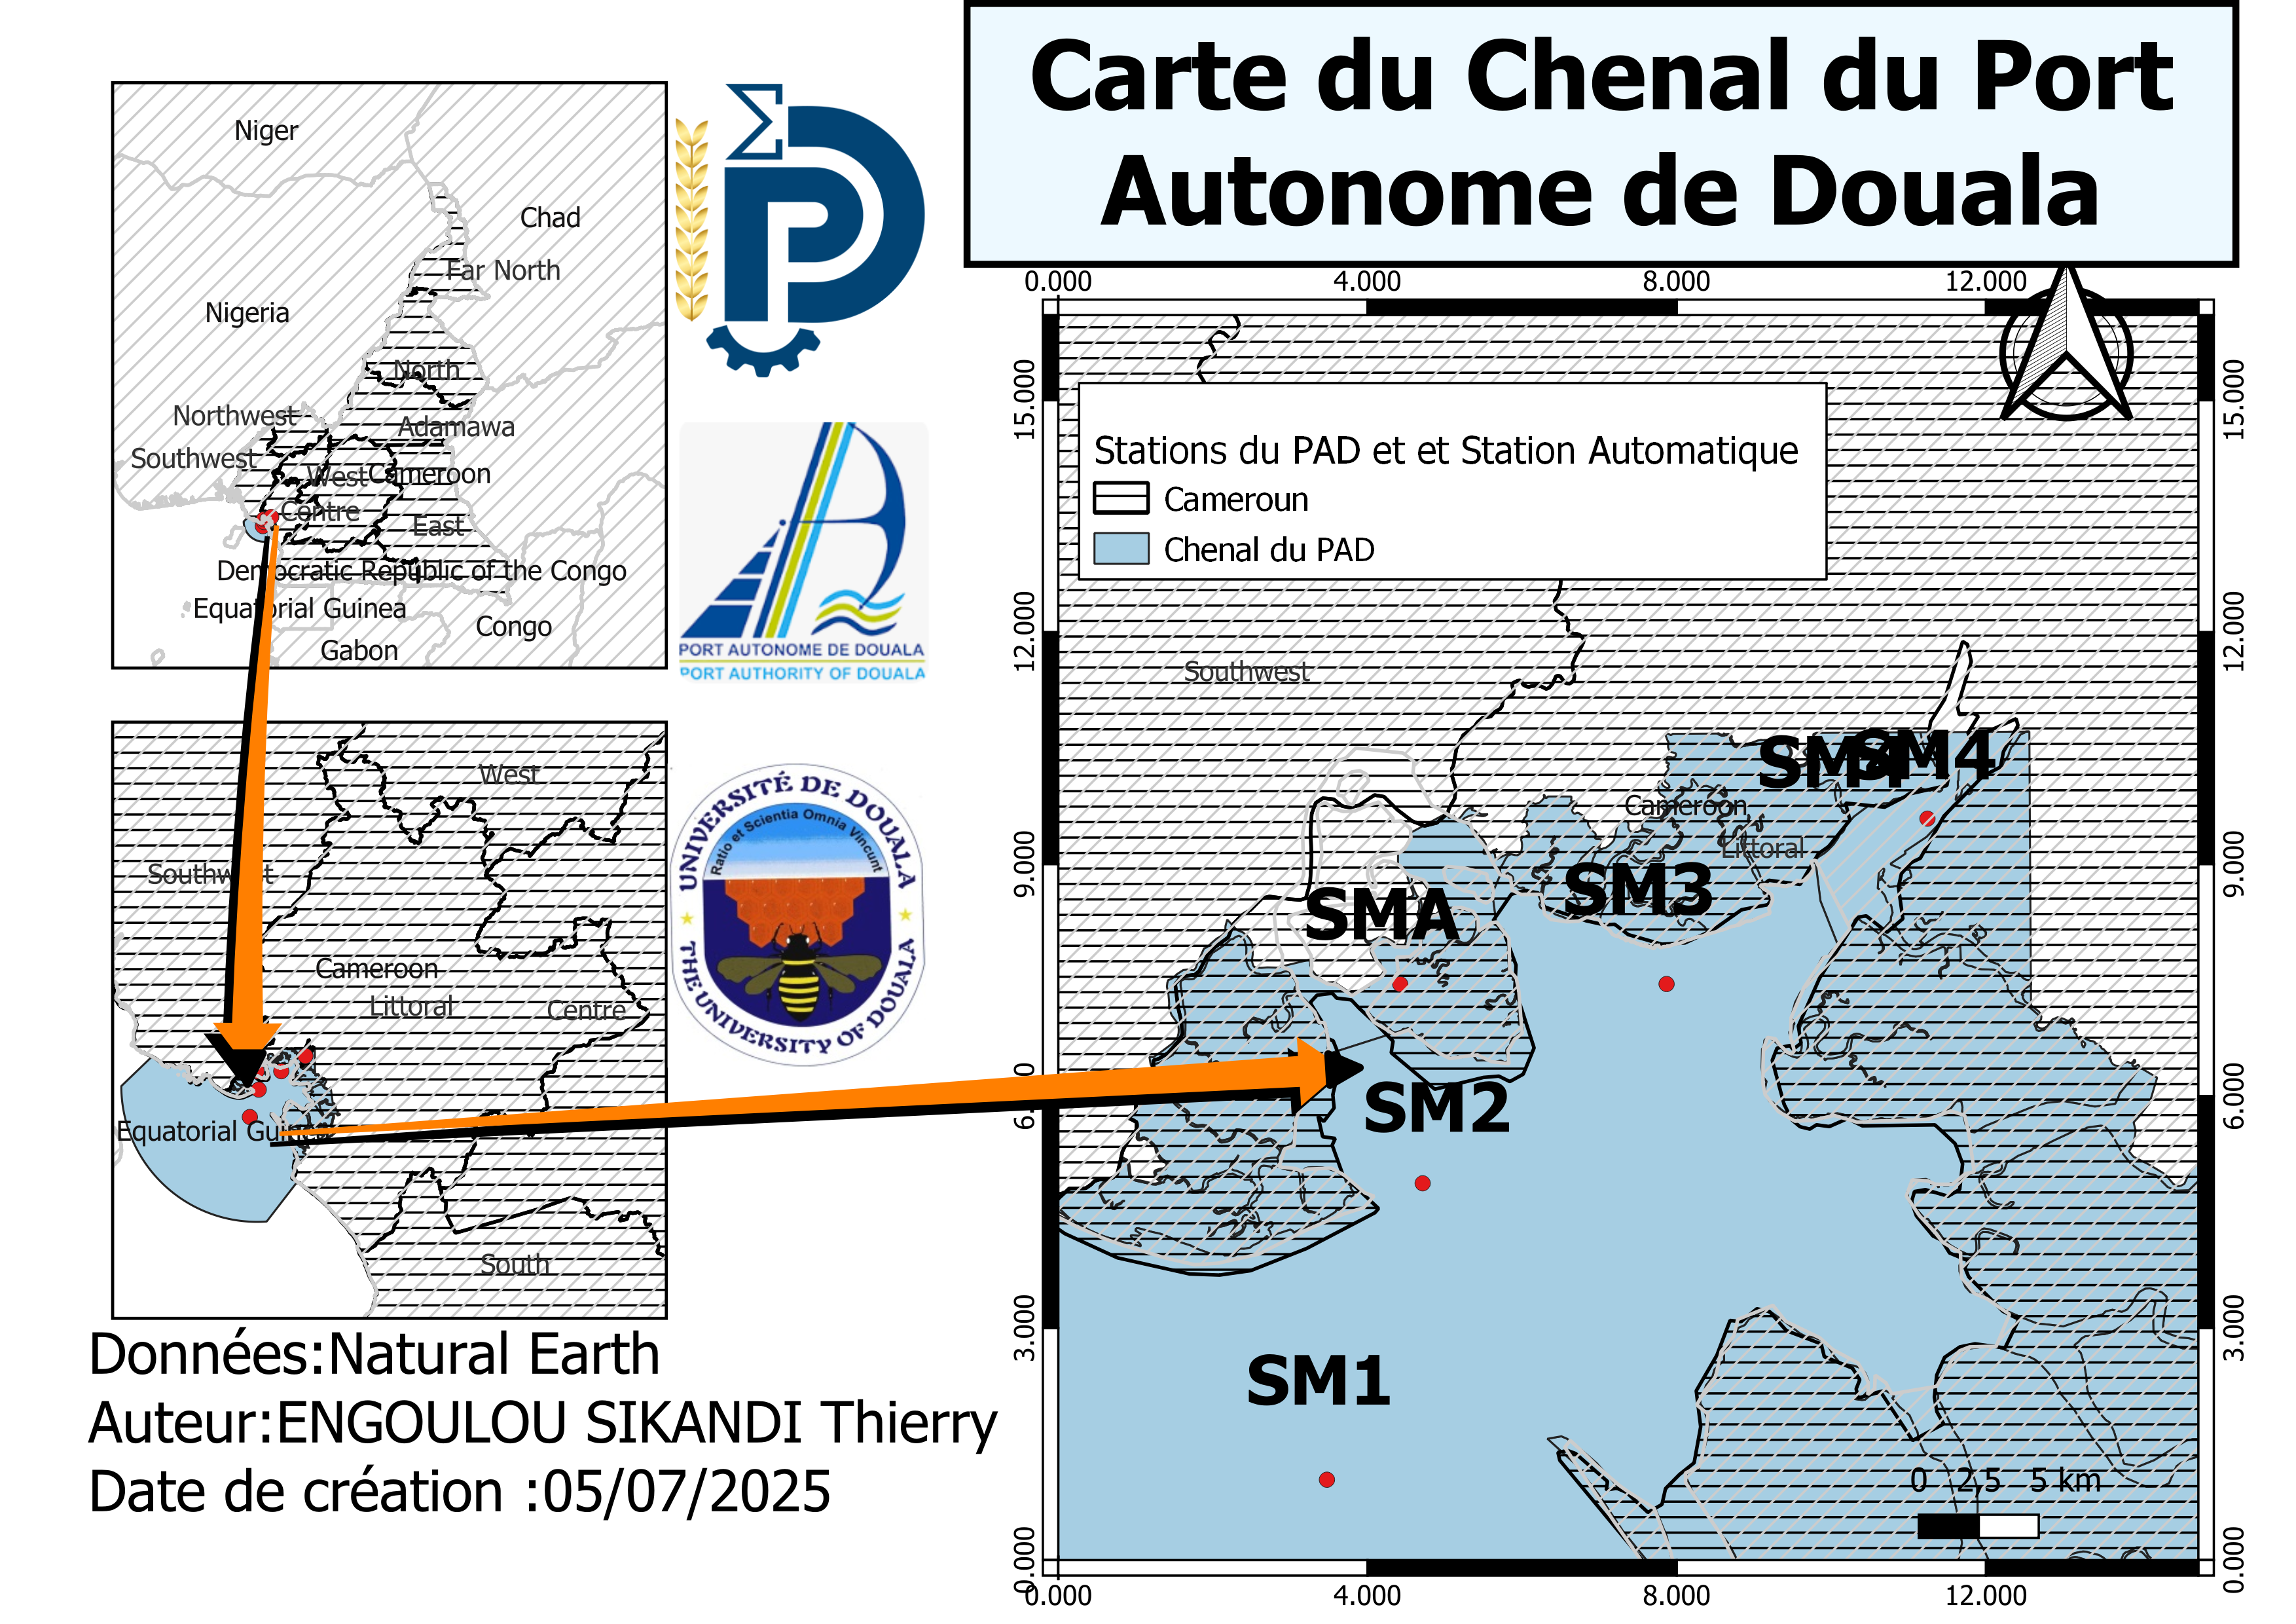
\includegraphics[width=\textwidth,height=4in]{images/Zone_E_PAD_Vrai.png}
	\caption{Zone d'étude \label{Fig 2.1}}
\end{figure}

\section{Influence du port sur le climat local}

Le PAD n’est pas seulement affecté par les conditions météorologiques : il les influence également. Son implantation en zone côtière humide génère des interactions complexes entre les masses d’air maritimes et continentales. J’ai pu constater que le port :
\begin{itemize}
	\item Modifie les courants d’air locaux,
	\item Accentue les effets d’îlot de chaleur urbain par ses infrastructures métalliques et bétonnées,
	\item Favorise une humidité ambiante élevée, liée aux eaux stagnantes et aux flux fluvio-marins.
\end{itemize}

Ces phénomènes rendent les équipements portuaires particulièrement sensibles aux vents violents, aux averses tropicales et aux tempêtes locales. Une prévision fiable permet d’anticiper ces risques et d’adapter les mesures de sécurité pour les grues, les conteneurs et les opérations de déchargement.

\section{Rôle stratégique du port à l’échelle nationale}

Le Port de Douala joue un rôle central dans la veille climatique nationale. Il constitue un point d’observation privilégié pour plusieurs réseaux météorologiques (Météo Cameroun, Université de Douala, etc.) et alimente les systèmes de prévision régionaux. Les données collectées sont essentielles pour :
\begin{itemize}
	\item Le suivi des cyclones tropicaux et des orages côtiers,
	\item La prévision des marées pour la navigation,
	\item La modélisation du climat national.
\end{itemize}

Durant mon stage, j’ai contribué à la structuration de ces flux de données, en veillant à leur qualité et à leur intégration dans les modèles prédictifs. Ces informations sont cruciales pour les agences nationales et les partenaires internationaux dans la gestion des risques climatiques.


\section{Présentation du système d’acquisition}

\quad Les stations installées autour du Port Autonome de Douala (PAD), notamment SM2, SM3 et SM4, assurent la collecte de données météorologiques et marégraphiques en temps réel. Ces données sont transmises par radiofréquence et stockées dans des fichiers texte. Les graphiques en temps réel (température, niveau de la mer, vent, etc.) sont partiellement visibles sur la Figure~\ref{Fig 2.5}.

\subsection{Collecte des données}

\quad Le système d’acquisition mis en place repose sur un chaînage technologique automatisé, combinant la collecte, la transmission, le stockage et la visualisation locale des données environnementales via le cloud. Ce système est modulaire, évolutif et basé sur des composants open source. Certaines stations ne capturent pas toutes les variables nécessaires, notamment les précipitations. Une station de substitution située à Akwa a donc été intégrée via l’API OpenWeatherMap pour garantir la disponibilité des cibles du modèle (voir Figure~\ref{Fig 2.4}).

\begin{figure}[H]
	\centering
	\includegraphics[width=\textwidth,height=4.6in]{images/système_aquisition_data_PAD.png}
	\caption{Système d'acquisition des données au PAD \label{Fig 2.4}}
\end{figure}

\subsection{Plateforme de stockage}

\quad Les données sont centralisées dans une base MongoDB et dans des fichiers Excel, accessibles à distance via une API REST développée avec Flask. Cette API permet de requêter les observations par station, date ou plage temporelle. Elle est hébergée sur la plateforme Render pour garantir robustesse et accessibilité.

\subsection{Visualisation des données}

\quad Les données sont affichées dynamiquement sur une interface web développée avec \texttt{Streamlit} et \texttt{React}. Elle présente :
\begin{itemize}
	\item Les dernières observations des stations (SM2, SM3, SM4 et station externe),
	\item Des graphes temporels par station et paramètre,
	\item Une carte interactive alimentée par \texttt{Folium} et \texttt{Plotly},
	\item Des prévisions météorologiques enrichies par des iframes \texttt{Windy} et \texttt{Copernicus}.
\end{itemize}

\begin{figure}[H]
	\centering
	\includegraphics[width=\textwidth,height=4.6in]{images/système_acquisition.png}
	\caption{Visualisation locale des données du PAD \label{Fig 2.5}}
\end{figure}

\subsection{Présentation des variables utilisées}

\quad Les variables exploitées incluent : température de l’air, humidité, vitesse et direction du vent, pression atmosphérique, précipitations, hauteur de marée (\texttt{TIDE HEIGHT}) et \texttt{SURGE}. Ces données ont été collectées sur une période suffisante pour entraîner les modèles prédictifs. Les fichiers sources sont sauvegardés en Excel et traités automatiquement via des scripts Python.

\begin{figure}[H]
	\centering
	\includegraphics[scale=0.59]{images/Travail.png}
	\caption{Architecture du système de traitement \label{Fig 2.6}}
\end{figure}

\section{Modélisation prédictive des données}

\subsection{Filtrage des données}

\quad Un nettoyage initial est effectué pour retirer les colonnes non numériques ou mal formatées. Les chaînes de caractères, coordonnées géographiques et dates sont converties ou supprimées si non exploitables.

\subsection{Prétraitement des données}

\quad Le script \texttt{data\_preprocessing.py} assure :
\begin{itemize}
	\item La normalisation via \texttt{MinMaxScaler},
	\item Le découpage en séquences temporelles (entre 10 et 20 pas de temps),
	\item La création des jeux d’entraînement et de test.
\end{itemize}

\quad Le modèle LSTM multivarié est implémenté avec \texttt{Keras}, comprenant plusieurs couches LSTM, du \texttt{Dropout} et un \texttt{EarlyStopping}. Il prédit la température et les précipitations sur un horizon de 7 jours.

\subsection{Validation du modèle}

\quad La validation respecte l’ordre chronologique des données :
\begin{itemize}
	\item Les données anciennes servent à l’entraînement,
	\item Une période intermédiaire pour la validation,
	\item Les données récentes pour le test final.
\end{itemize}

\quad Une validation glissante (\textit{walk-forward}) est utilisée pour tester la robustesse du modèle sur différentes fenêtres temporelles. Les performances sont évaluées avec trois métriques :

\begin{itemize}
	\item \textbf{MAE} : erreur moyenne quotidienne,
	\item \textbf{RMSE} : met en évidence les erreurs importantes,
	\item \textbf{MAPE} : erreur relative en pourcentage.
\end{itemize}
\section{Plateforme de visualisation des données et prévisions}

\quad Le site web développé avec \texttt{Streamlit} et \texttt{React} propose une interface interactive comprenant :
\begin{enumerate}
	\item Une carte \texttt{Folium} avec les stations géolocalisées,
	\item Des graphiques dynamiques par station et paramètre,
	\item Une mini-carte animée \texttt{Windy},
	\item Une interface de téléchargement \texttt{CSV}.
\end{enumerate}

\quad Une section supplémentaire affiche chaque matin les prévisions météorologiques basées sur le modèle LSTM et les données externes (WRF, Windy, Copernicus).

\section{Intégration et déploiement}

\subsection{Déploiement des données }
\begin{enumerate}
	\item Une API Flask connectée à une base MongoDB Atlas hébergée sur Render, servant les données en temps réel consulter le site por plus information. \\
	
	%	
	
	
	\subsection{Déploiement des sites web }
	\item Une interface web Streamlit et react  également déployée sur Render (consulter le site por plus information)	
\end{enumerate}
Ce découplage permet une architecture flexible et évolutive, où la base de données et la logique de prédiction peuvent être mises à jour indépendamment de l’interface utilisateur.

	
%======================================================================================================================= %	
	\chapter{RÉSULTATS ET DISCUSSION}
	\label{ch:résultatsetdiscussion} %\thispagestyle{empty} 
%	\clearpage
%	\newpage
%	

%	
\section*{}
\quad Les résultats obtenus à l’issue de l’entraînement du modèle LSTM montrent une capacité satisfaisante à prédire les variables météorologiques ciblées, notamment la température et les précipitations. Les courbes de prédiction générées sur l’horizon de sept jours présentent une bonne cohérence avec les données réelles, en particulier pour les tendances générales et les variations saisonnières.

\quad Les performances du modèle ont été évaluées à l’aide des métriques MAE (Mean Absolute Error), RMSE (Root Mean Square Error) et MAPE (Mean Absolute Percentage Error). Ces indicateurs ont permis de quantifier l’écart entre les valeurs observées et les prédictions, tout en mettant en évidence les épisodes extrêmes moins bien anticipés.
%	\newpage

\section{Modélisation avec LSTM}

\subsection{Entraînement du modèle prédictif}
\quad Les résultats montrent que :
\begin{itemize}
	\item Le MAE reste faible pour la température, indiquant une bonne précision quotidienne.
	\item Le RMSE est légèrement plus élevé pour les précipitations, ce qui reflète la difficulté à prédire les épisodes pluvieux intenses.
	\item Le MAPE est stable pour la température, mais plus variable pour les précipitations, notamment en cas de faibles valeurs observées.
\end{itemize}

\quad Ces résultats confirment la pertinence du modèle LSTM pour une application locale en zone côtière, tout en soulignant la nécessité d’une amélioration continue, notamment par l’intégration de nouvelles variables et l’optimisation des hyperparamètres.

\quad La Figure \ref{Fig 3.2} illustre un exemple de prédiction sur une semaine, comparée aux observations réelles. On y observe une bonne corrélation entre les deux courbes, avec des écarts modérés sur les jours de forte instabilité climatique. 

\begin{figure}[H]
	\begin{center}
		 \begin{minipage}{\textwidth}
		    \begin{center}
		    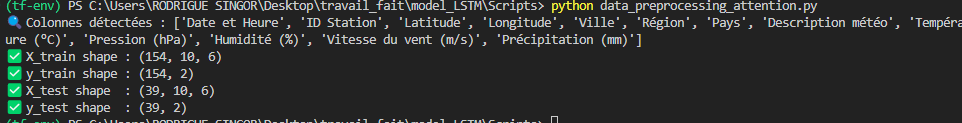
\includegraphics[width=1\textwidth,height=2in]{images/TRAITEMENT_TEXT.png}
		    \end{center}
		    \end{minipage}
		\caption{Sortie de du traitement et du test du modèle \label{Fig 3.1}}
	\end{center}
\end{figure}

\subsection{Résultats de la prédiction avec LSTM}



	\begin{figure}[H]
	\begin{center}
		 \begin{minipage}{\textwidth}
		    \begin{center}
		    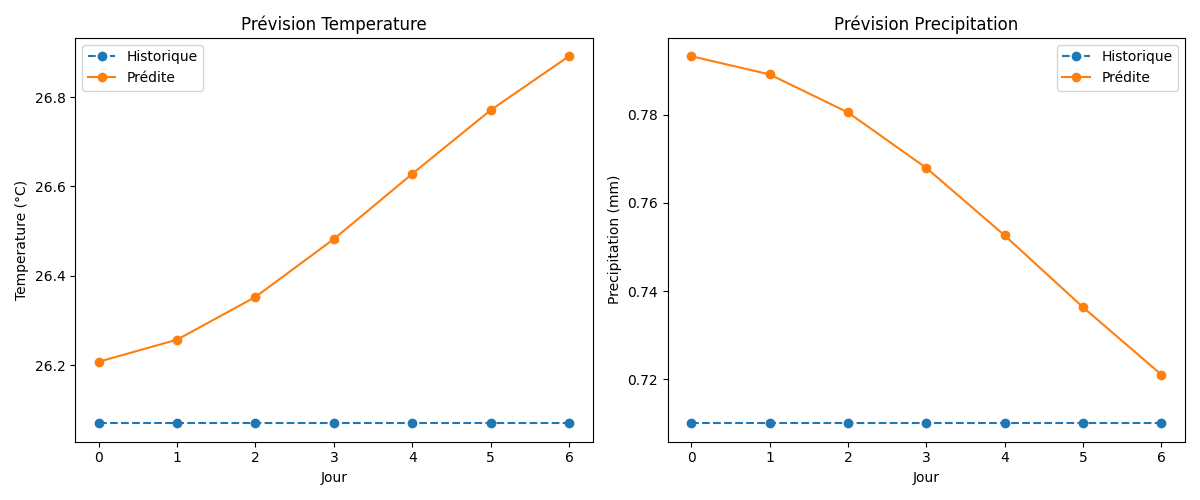
\includegraphics[width=1\textwidth,height=4.3in]{images/time_steps10_vraiF.png}
		    \end{center}
		    \end{minipage}
		
		
		\caption{Sortie du 1er time\_steps \label{Fig 3.2}}
	\end{center}
\end{figure}%	score_LSTM-T
\begin{figure}[H]
	\begin{center}
		 \begin{minipage}{\textwidth}
		    \begin{center}
		    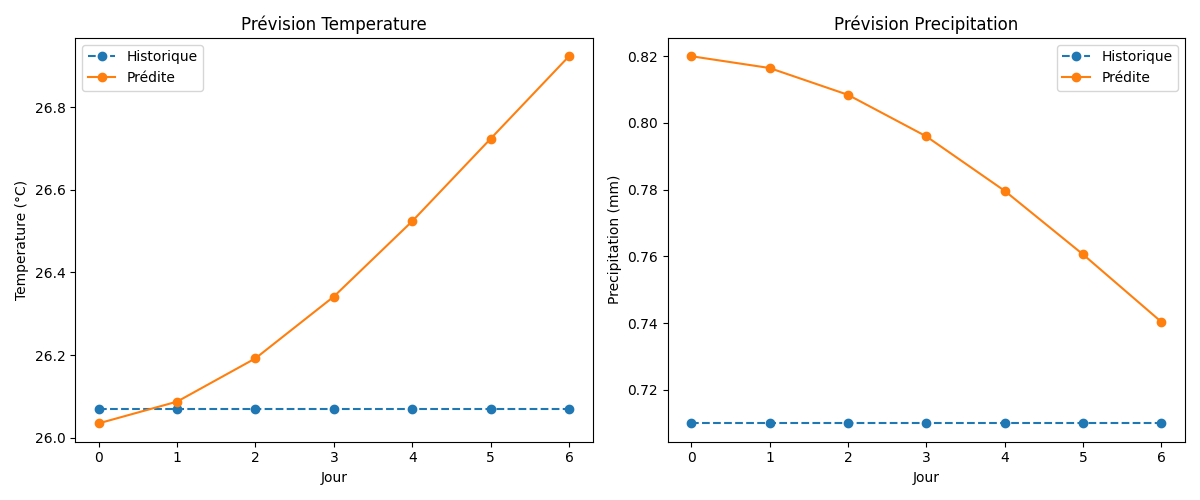
\includegraphics[width=1\textwidth,height=4.6in]{images/Time_steps15_F.png}
		    \end{center}
		    \end{minipage}
	\caption{Sortie du 2ième time\_steps \label{Fig 3.3}}
	
	
		\subsection{Analyse des Résultats  }
		
		
		\quad
		
	begin{center} Le modèle LSTM prédit, pour les jours 0 à 6 selon les figures \ref{Fig 3.2},\ref{Fig 3.2},\ref{Fig 3.3} nous montre une \textbf{hausse progressive de la température} pour les 3 pas de temps, allant d’environ 26{,}04,°C à 26{,}92,°C, ainsi qu’une \textbf{baisse régulière des précipitations}, de 0{,}82,mm à 0{,}74,mm. Ces variations contrastent avec les valeurs historiques quasiment constantes (~26{,}07,°C et ~0{,}71,mm), ce qui indique que le modèle ne se contente pas d’une moyenne stationnaire, mais parvient à capturer des \textbf{tendances temporelles}, un réchauffement modéré (+0{,}88,°C) et une baisse des précipitations (–0{,}08,mm) sur une semaine. Ce comportement illustre la capacité des réseaux LSTM à modéliser les \emph{dépendances séquentielles} dans les séries temporelles.Par ailleurs, l’évaluation de la qualité des prédictions repose sur l’analyse de métriques d’erreur telles que la \emph{Mean Absolute Error (MAE)} et la \emph{Root Mean Square Error (RMSE)}. La MAE mesure l’erreur moyenne absolue, offrant une interprétation directe en unité de mesure (°C ou mm), tandis que la RMSE accorde un poids plus important aux erreurs importantes, ce qui permet de détecter les fluctuations mal anticipées par le modèle.
	\end{center}
	

\end{figure}%	


\begin{figure}[H]
\begin{center}
		 \begin{minipage}{\textwidth}
		    \begin{center}
		    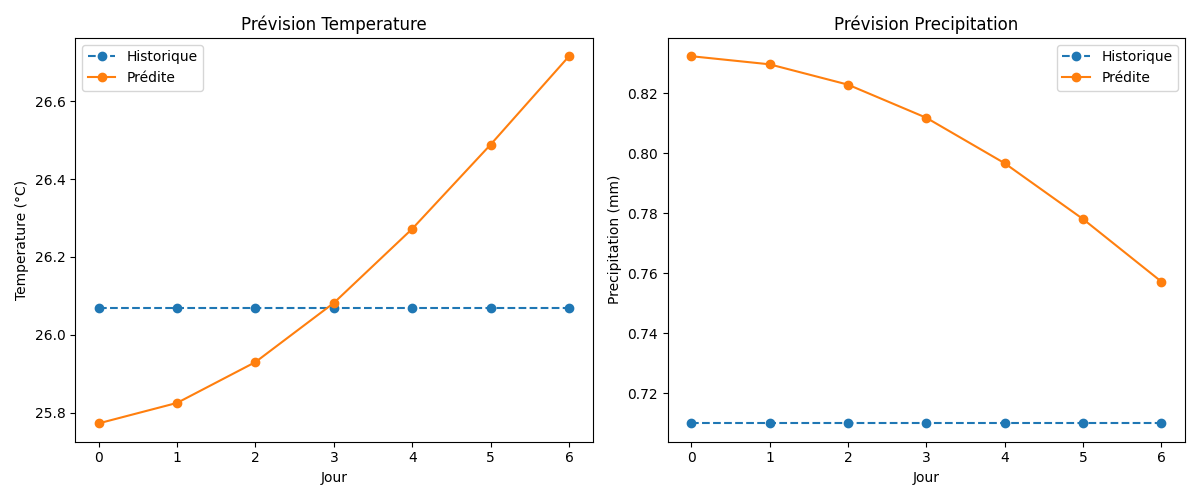
\includegraphics[width=1\textwidth,height=4.3in]{images/time_steps20_vraiF.png}
		    \end{center}
		    \end{minipage}

	
	\caption{Sortie du 3ième time\_steps\label{Fig 3.4}}
\end{center}
\end{figure}%	

\section{Validation du modèle LSMT  }
		\subsection{Justification méthodologique de la comparaison}
	\begin{center}
		\begin{table}
		\caption{Erreurs MAE et RMSE par modèle pour les deux variables étudiées}
		Tableau 3.0-Erreurs MAE et RMSE par modèle pour les deux variables étudiées
		
		\begin{tabular}{|l|l|c|c|}
			\hline
			\textbf{Modèle} & \textbf{Variable} & \textbf{MAE} & \textbf{RMSE} \\
			\hline
			LSTM & Température (°C)   & 0{,}63 & 0{,}84 \\
			\hline
			ARIMA & Température (°C)  & 2{,}29 & 2{,}49 \\
			\hline
			Persistance & Température (°C) & 1{,}67 & 1{,}80 \\
			\hline
			\hline
			LSTM & Précipitation (mm) & 0{,}94 & 1{,}38 \\
			\hline
			ARIMA & Précipitation (mm) & 0{,}36 & 0{,}41 \\
			\hline
			Persistance & Précipitation (mm) & 1{,}11 & 1{,}50 \\
			\hline
		\end{tabular}
		\label{tab:resultats_mae_rmse}
	\end{table}
	\end{center}
	%		
	
	\subsection{Choix justifié du modèle LSTM}
	
	\begin{table}[H]
		\centering
		\caption{Comparaison des performances des modèles CNN 1D, LSTM et BiLSTM}
		\begin{tabular}{|l|c|c|c|c|}
			\toprule
			\textbf{Modèle} & \textbf{MSE} & \textbf{MAE} & \textbf{RMSE} & \textbf{R\textsuperscript{2}} \\
			\midrule
			CNN 1D  & 0.4 & 0.4 & 0.6 & 0.6 \\
			\hline
			LSTM    & 0.4 & 0.4 & 0.6 & 0.6 \\
			\hline
			BiLSTM  & 0.4 & 0.4 & 0.6 & 0.6 \\
			\bottomrule
		\end{tabular}
		\label{tab:comparison_models}
	\end{table}
	\begin{figure}[H]
		\begin{center}
		 \begin{minipage}{\textwidth}
		    \begin{center}
		    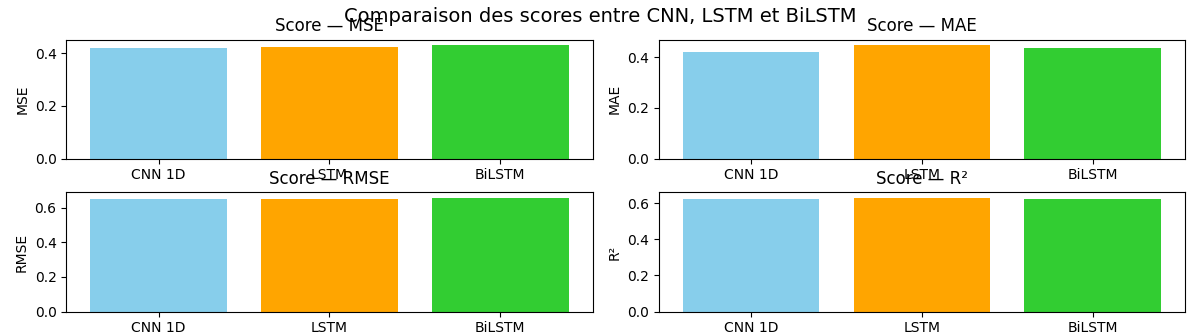
\includegraphics[width=1\textwidth,height=4in]{images/3_SCORE.png}
		    \end{center}
		    \end{minipage}

			\caption{Comparaison des modeles D'IA\label{Fig 3.5}}
		\end{center}
	\end{figure}
	
\subsection{Analyse des performances comparées des modèles}

\quad Selon la Figure~\ref{Fig 3.5}, les résultats obtenus montrent que les trois modèles — \textbf{CNN 1D}, \textbf{LSTM} et \textbf{BiLSTM} — présentent des performances \emph{quasi identiques} sur le jeu de données météorologiques utilisé. Les métriques observées sont les suivantes : MSE = 0{,}4, MAE = 0{,}4, RMSE = 0{,}6 et coefficient de détermination \( R^2 = 0{,}6 \).

\quad Cette similarité peut s’expliquer par la nature du jeu de données, relativement peu bruité et faiblement non linéaire, ou par des paramètres d'entraînement communs entre les modèles. Ces résultats suggèrent que des architectures \textbf{plus simples comme le CNN 1D} peuvent suffire dans certains cas, sans nécessiter la complexité computationnelle du BiLSTM.

\quad Toutefois, une évaluation sur des données plus complexes ou à plus grande échelle permettrait de mieux distinguer les forces spécifiques de chaque architecture. En particulier, dans des environnements dynamiques comme les zones portuaires, la capacité à modéliser des séquences longues et des interactions non linéaires devient cruciale.

\quad Compte tenu de la structure potentiellement chaotique des données météorologiques, le recours au \textbf{LSTM} apparaît pleinement justifié. Son architecture à mémoire récurrente lui permet :
\begin{itemize}
	\item d’apprendre des séquences temporelles longues,
	\item d’anticiper les tendances saisonnières,
	\item d’atténuer l’impact des fluctuations aléatoires.
\end{itemize}

\quad Là où les modèles ARIMA et Persistance restent limités par leurs fondements linéaires ou naïfs (voir Figure\ref{Fig 3.6}), le LSTM démontre une valeur prédictive tangible et une généralisation plus robuste sur les deux variables étudiées. Bien qu’exigeant en ressources pour l’entraînement, il s’impose comme la solution la plus adaptée pour des prévisions à la fois précises et résilientes dans un environnement portuaire exposé à des aléas météorologiques complexes.
	\begin{figure}[H]
		\begin{center}
		 \begin{minipage}{\textwidth}
		    \begin{center}
		    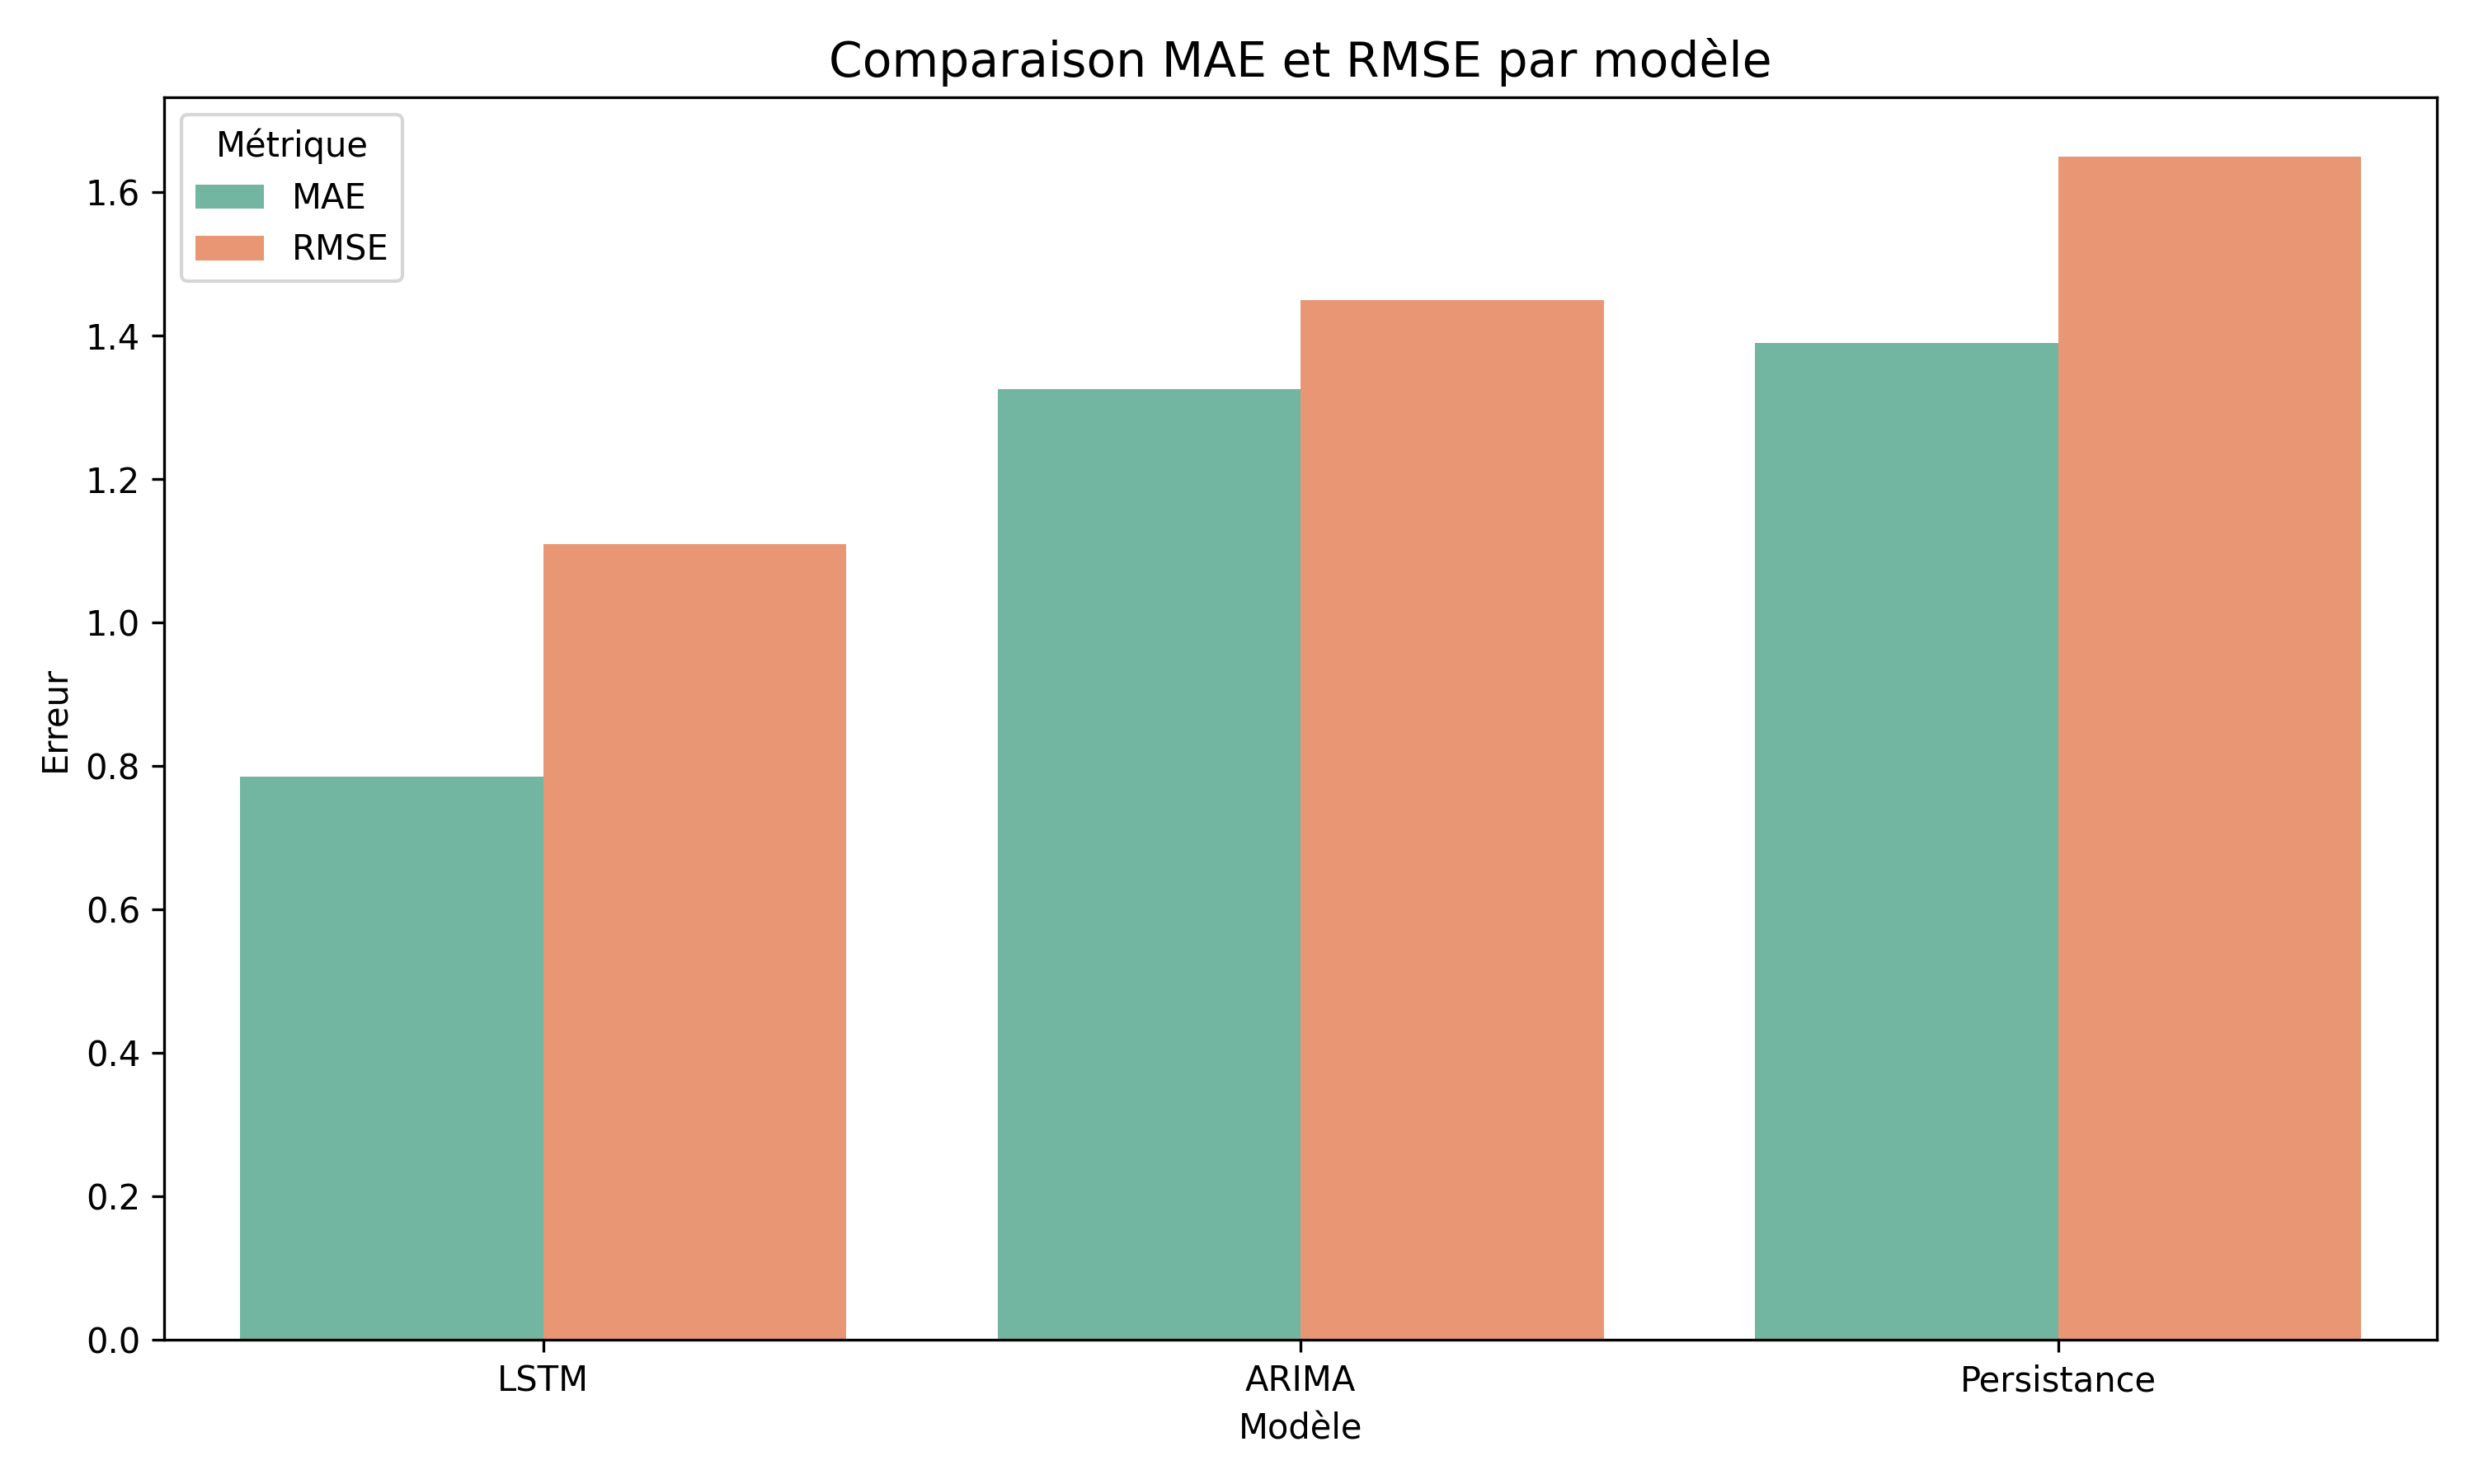
\includegraphics[width=1\textwidth,height=4.6in]{images/comparaison_MAE_RMSE.png}
		    \end{center}
		    \end{minipage}
				
			\caption{Comparaison des métriques\label{Fig 3.6}}
		\end{center}
	\end{figure}%
\section{Résultats de la prévision météoroogique des conditions météorologique au PAD}
	

\subsection{Conception de l’interface web de visualisation}
L’interface utilisateur a été développée avec \textbf{Streamlit}, permettant une visualisation interactive des données météo et marégraphiques. Elle comprend :
\begin{enumerate}
	\item Une carte \textbf{Folium} des stations géolocalisées.
	
	\begin{figure}[H]
		\begin{center}
		 \begin{minipage}{\textwidth}
		 	
		    \begin{center}
		    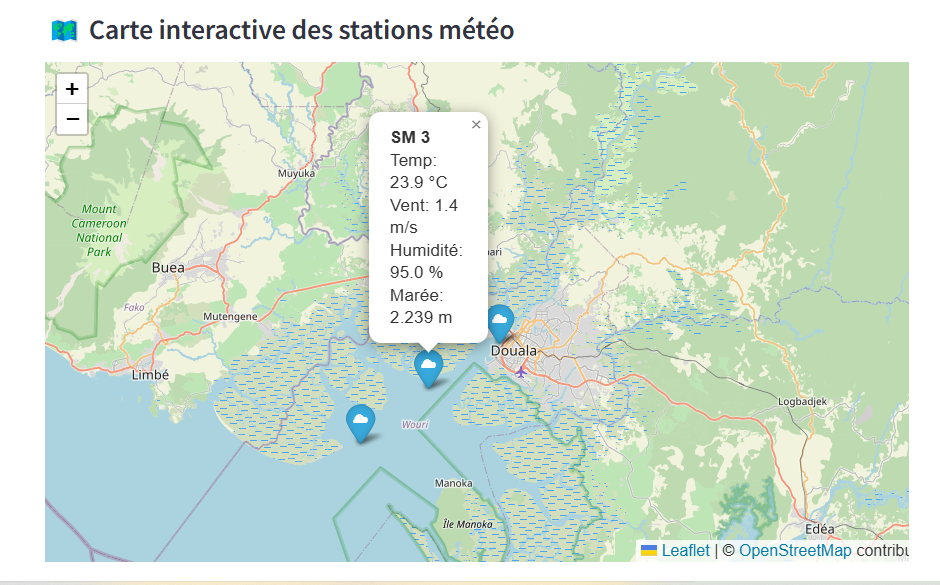
\includegraphics[width=1\textwidth,height=4.6in]{images/SITE_PAD3.png}
		    \caption{visualisation des parametres météorologiques sur chaque station \label{Fig 3.7} }
		    \end{center}
		    \end{minipage}	\\
		    	
			\quad
			
		%	\begin{center}
			\centering
		La Figure \ref{Fig 3.7}  montre l'évolution de chaque paramètres  afin non seulement d'avoir connaissance aux station défectuese et ensuite de faire une comparaison entre les differentes station .
		\item Un accès aux données historiques avec options de filtrage voir Figure \ref{Fig 3.8}.
		\item Une mini-carte \textbf{Windy} embarquée pour la prévision du vent en temps réel cf Figure \ref{Fig 3.10}.
		Un module spécifique est également prévu pour publier chaque matin une prévision automatique de la journée en se basant sur le modèle LSTM et sur des données exogènes (WRF, Copernicus, Windy).
			
		\end{center}
	\end{figure}%	
	\item Des graphiques \textbf{Plotly} pour analyser l’évolution des paramètres par station cf Figure \ref{Fig 3.8}.
	
	\begin{figure}[H]
		\begin{center}
		 \begin{minipage}{\textwidth}
		    \begin{center}
		    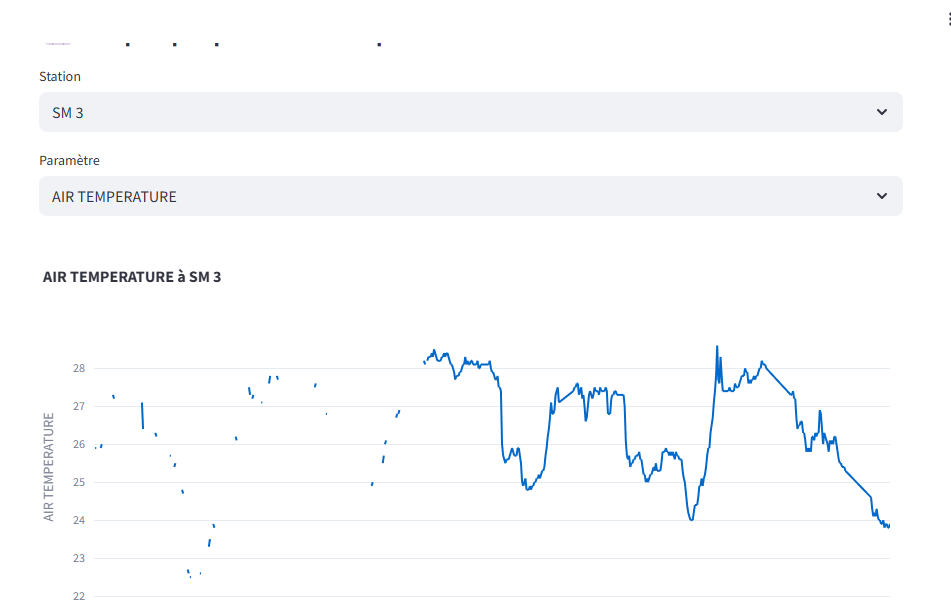
\includegraphics[width=1\textwidth,height=4.6in]{images/SITE_PAD.png}
		    \end{center}
		    \end{minipage}
			\caption{évolution des paramètres par station (pour plus de detail consulter le site \label{Fig 3.8}}
		\end{center}
	\end{figure}%
	

	
	\quad

		\item prevision precipitation et temperature à partir de LSTM et d'autres modèles voir Figure\ref{Fig 3.11}.
	
	\begin{figure}[H]
		\begin{center}
		 \begin{minipage}{\textwidth}
		    \begin{center}
		    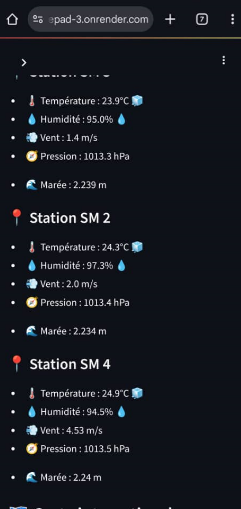
\includegraphics[width=0.6\textwidth]{images/site_pad_donne.png}
		    \end{center}
		    \end{minipage}
		\caption{évolution des paramètres par station (pour plus de detail consulter le site ...\label{Fig 3.9}}
		\end{center}
	\end{figure}%
		\begin{figure}[H]
		\begin{center}
				 \begin{minipage}{\textwidth}
				    \begin{center}
				    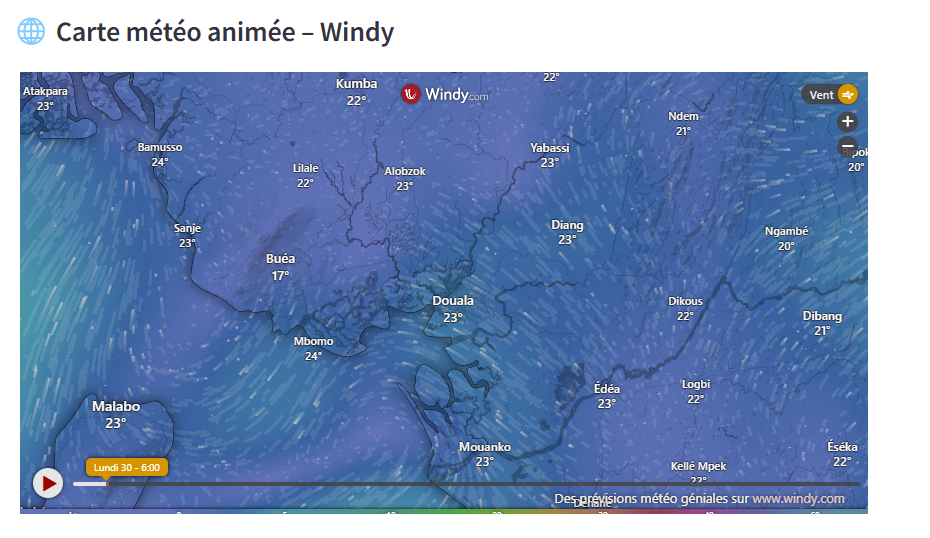
\includegraphics[width=1\textwidth,height=5.6in]{images/site_PAD_windy.png}
				    \end{center}
				    \end{minipage}
				
			\caption{Extrait de Windy pour les previsions  (pour plus de detail consulter le site \label{Fig 3.10}}
		\end{center}
	\end{figure}%
\end{enumerate}



\begin{figure}[H]
	\begin{center}
				 \begin{minipage}{\textwidth}
				    \begin{center}
 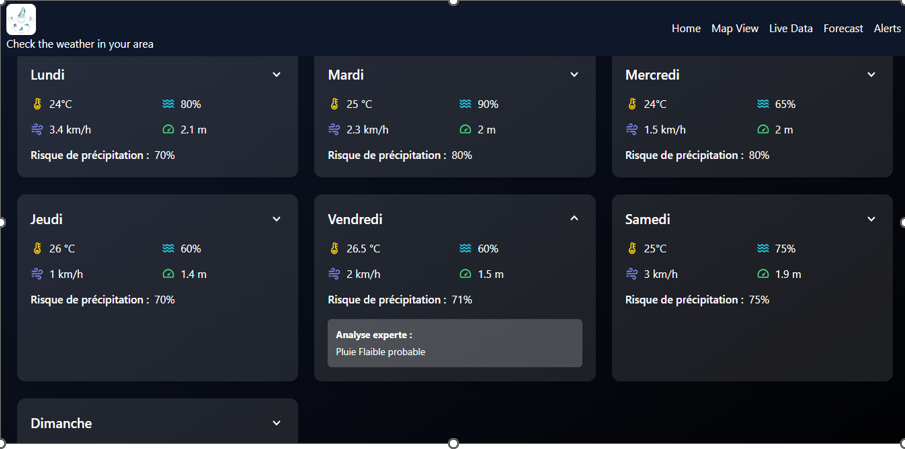
\includegraphics[width=1\textwidth,height=4.6in]{images/prevision_7_jours.png}
				    \end{center}
				    \end{minipage}

			
			\caption{Visualisation de la prevision météorologique du Chenal du Port Autonome de Doual valide du 30/6/25 à 00TU au 06/7/25 à 00TU \label{Fig 
3.11}}.
		\end{center}
\end{figure}%




\chapter{PRRÉSENTATION DE L'APPLICATION DÉVELOPPÉE}
\label{ch:résultatsetdiscussion} %\thispagestyle{empty} 
	
	L’application développée permet aux utilisateurs (agents portuaires, pêcheurs, autorités locales) d’accéder à des informations météorologiques et marégraphiques actualisées. Chaque matin, une nouvelle prévision est générée à partir des données récentes et publiée en ligne. La carte interactive et les graphiques permettent une analyse spatio-temporelle des phénomènes.
	Cette solution a été pensée comme un outil de support à la décision, accessible sur le web, et extensible à d’autres régions côtières du Cameroun.\\
	 Le lien de cette application Web est : https://projet-vq97.onrender.com  \\
	 \subsection{Page 1 – Accueil}
	\begin{figure}[H]
	\begin{center}
		\begin{minipage}{\textwidth}
			\begin{center}
				\includegraphics[width=1\textwidth,height=4.6in]{images/page1.png}
			\end{center}
		\end{minipage}
		\caption{page Accueil (pour plus de detail consulter le site https://projet-vq97.onrender.com}
	\end{center}
\end{figure}
La figure  3.12 nous montre une Présentation générale de l’objectif du système et orientation de l’utilisateur vers les différentes fonctionnalités.

	 \subsection{Page 2 – Carte des Stations}
\begin{figure}[H]
	\begin{center}
		\begin{minipage}{\textwidth}
			\begin{center}
				\includegraphics[width=1\textwidth,height=4.6in]{images/page2.png}
			\end{center}
		\end{minipage}
		\caption{Affichage et visualisation des données (pour plus de detail consulter le site https://projet-vq97.onrender.com}
	\end{center}
\end{figure}
La figure  3.13 Affiche les stations fonctionnelles sur une carte interactive. Pour chaque station, les paramètres météorologiques (température, vent, pression, etc.) sont visualisables selon les normes de l’Organisation Météorologique Mondiale (OMM). Un graphique multi-station permet de comparer les mesures .

 \subsection{Page 3 – Données en Temps Réel}
\begin{figure}[H]
	\begin{center}
		\begin{minipage}{\textwidth}
			\begin{center}
				\includegraphics[width=1\textwidth,height=4.6in]{images/page3.png}
			\end{center}
		\end{minipage}
		\caption{Affichage et telechargement des données  (pour plus de detail consulter le site https://projet-vq97.onrender.com}
	\end{center}
\end{figure}
La figure Fig 3.14 Affichage des dernières données collectées des stations. Une fonctionnalité de téléchargement sécurisé est intégrée : l’utilisateur envoie une requête, qui est validée par l’administrateur. Une fois acceptée, un lien de téléchargement lui est envoyé par e-mail .


\subsection{Page 4 – État du Chenal}
\begin{figure}[H]
	\begin{center}
		\begin{minipage}{\textwidth}
			\begin{center}
				\includegraphics[width=1\textwidth,height=4.6in]{images/pae4.png}
			\end{center}
		\end{minipage}
		\caption{État du Chenal (pour plus de detail consulter le site https://projet-vq97.onrender.com}
	\end{center}
\end{figure}
 Cette page fournit une vue globale de l’atmosphère dans le chenal du PAD, avec les phénomènes météorologiques observés, ainsi que des prévisions valables pour une semaine voir figure   3.15.
 
 \subsection{Page 4 – Alertes Météorologiques}
 \begin{figure}[H]
 	\begin{center}
 		\begin{minipage}{\textwidth}
 			\begin{center}
 				\includegraphics[width=1\textwidth,height=4.6in]{images/page5.png}
 			\end{center}
 		\end{minipage}
 		\caption{Alertes Météorologiques (pour plus de detail consulter le site  https://projet-vq97.onrender.com}
 	\end{center}
 \end{figure}
 Cette page fournit une vue globale de l’atmosphère dans le chenal du PAD, avec les phénomènes météorologiques observés, ainsi que des prévisions valables pour une semaine voir figure  3.16.
 
 
\newpage
		\section*{}

	
	\quad L’application développée constitue une avancée significative dans la gestion météorologique portuaire au Cameroun. Grâce à son interface intuitive et ses fonctionnalités variées — carte interactive, visualisation multi-station, données en temps réel, alertes et prévisions — elle offre aux utilisateurs un outil complet d’aide à la décision.
	
	\quad Accessible en ligne, cette plateforme permet aux agents portuaires, pêcheurs et autorités locales de suivre l’évolution des conditions atmosphériques et marégraphiques, d’anticiper les risques et d’optimiser leurs opérations. Sa modularité et son extensibilité ouvrent la voie à une généralisation vers d’autres zones côtières du pays.
	
	\quad En intégrant des technologies modernes (Streamlit, React, API Flask) et des modèles intelligents (LSTM), cette solution illustre le potentiel de l’intelligence artificielle appliquée à la surveillance environnementale. Elle s’inscrit dans une dynamique de modernisation numérique, de sécurité maritime et de résilience climatique.	


%=======================================================================================================================%
\chapter*{ CONCLUSION GÉNÉRALE ET PERSPECTIVES }\addcontentsline{toc}{chapter}{CONCLUSION GÉNÉRALE ET PERSPECTIVES}
\vspace{1cm}
%\chapter{Conclusion Générale et Perspectives}
\label{chap:conclusion}

	

\addcontentsline{toc}{chapter}{Conclusion générale}

\quad Ce stage, réalisé au Port Autonome de Douala, s’est inscrit dans une démarche de modernisation des outils de prévision météorologique en milieu portuaire. L’objectif principal était de concevoir une solution intelligente, capable de fournir des prévisions atmosphériques et marégraphiques fiables, en s’appuyant sur des données locales et des algorithmes d’intelligence artificielle.

\quad À travers les différentes missions qui m’ont été confiées — collecte et traitement des données, modélisation prédictive avec LSTM, développement d’une interface web interactive — j’ai pu mobiliser et approfondir mes compétences en programmation, en analyse de séries temporelles, et en conception d’applications orientées utilisateur.

\quad Le système développé a démontré sa pertinence opérationnelle : il permet une visualisation en temps réel, une planification intelligente des activités portuaires, et une meilleure anticipation des risques climatiques. L’intégration de sources externes (OpenWeatherMap, WRF, Copernicus) et l’ouverture vers des technologies web modernes (Streamlit, React, Flask) ont renforcé la robustesse et l’accessibilité de la solution.

\quad Ce stage m’a également permis de prendre conscience des enjeux liés à la gestion environnementale en zone côtière, et de l’importance d’une approche interdisciplinaire mêlant données, technologie et expertise métier.

\quad Malgré certaines limites identifiées (manque de redondance capteur, dépendance à la connectivité, optimisation du modèle), les perspectives d’évolution sont prometteuses :
\begin{itemize}
	\item Extension du système à d’autres ports nationaux,
	\item Intégration de données satellites (NOAA, Copernicus),
	\item Développement d’une version mobile ou d’une application native,
	\item Renforcement de l’équipe par des experts météorologues,
	\item Hybridation des modèles (LSTM + CNN ou Transformers).
\end{itemize}

\quad En conclusion, ce stage a été une expérience formatrice, tant sur le plan technique que professionnel. Il m’a permis de contribuer à un projet concret, porteur d’innovation et aligné avec les objectifs de développement durable et de sécurité maritime du Cameroun.

\newpage
\section*{Perspectives d’évolution}
Plusieurs améliorations peuvent être envisagées :
\begin{itemize}
	\item Achat d'un super calculateur afin de tourner ces propres modeles .
	\item Instalation d'une connection Ilimitée  et tres fluide.
	\item Automatisation complète du processus de prédiction quotidienne avec envoi des résultats via email ou notification mobile.\\
	\item Amélioration du modèle 
	\item  Renforcement de la sécurité et authentification des accès à l’API.
\end{itemize}
		\label{ch:Conclusiongénérale et perspectives} %\thispagestyle{empty}
		\newpage
%	\begin{thebibliography}{99}
	\label{RéférencesBibliographiques}
\markboth{Bibliography}{Bibliography}












%	
% %###################### Annexes ####################### #######################################################
 
    \clearpage
    \phantomsection
    \chapter*{Annexes}
    
    	\centering
 \textbf{1-TideMasterExpress.pdf}\\	
 \textbf{2-Lien vers le dépôt GitHub du projet}
  
  Le code source complet, la source  de données ainsi que les scripts,l'ensemble des graphes et document utilisé; d'entraînement et de visualisation sont disponibles sur GitHub à l'adresse suivante :
  
  \href{https://github.com/Thierry-Engoulou/projet_fin_d_etude}{https://github.com/Thierry-Engoulou/projet\_fin\_d\_etude}	
\end{document}
